% Options for packages loaded elsewhere
\PassOptionsToPackage{unicode}{hyperref}
\PassOptionsToPackage{hyphens}{url}
\PassOptionsToPackage{dvipsnames,svgnames,x11names}{xcolor}
%
\documentclass[
  12pt,
  a4paper,
]{article}
\title{\singlespacing \vspace{-1.6cm} \LARGE Covariation among reproductive traits in flowering plants determine interactions with floral visitors}
\author{}
\date{\vspace{-2.5em}}

\usepackage{amsmath,amssymb}
\usepackage[]{mathpazo}
\usepackage{setspace}
\usepackage{iftex}
\ifPDFTeX
  \usepackage[T1]{fontenc}
  \usepackage[utf8]{inputenc}
  \usepackage{textcomp} % provide euro and other symbols
\else % if luatex or xetex
  \usepackage{unicode-math}
  \defaultfontfeatures{Scale=MatchLowercase}
  \defaultfontfeatures[\rmfamily]{Ligatures=TeX,Scale=1}
\fi
% Use upquote if available, for straight quotes in verbatim environments
\IfFileExists{upquote.sty}{\usepackage{upquote}}{}
\IfFileExists{microtype.sty}{% use microtype if available
  \usepackage[]{microtype}
  \UseMicrotypeSet[protrusion]{basicmath} % disable protrusion for tt fonts
}{}
\makeatletter
\@ifundefined{KOMAClassName}{% if non-KOMA class
  \IfFileExists{parskip.sty}{%
    \usepackage{parskip}
  }{% else
    \setlength{\parindent}{0pt}
    \setlength{\parskip}{6pt plus 2pt minus 1pt}}
}{% if KOMA class
  \KOMAoptions{parskip=half}}
\makeatother
\usepackage{xcolor}
\IfFileExists{xurl.sty}{\usepackage{xurl}}{} % add URL line breaks if available
\IfFileExists{bookmark.sty}{\usepackage{bookmark}}{\usepackage{hyperref}}
\hypersetup{
  pdftitle={ Covariation among reproductive traits in flowering plants determine interactions with floral visitors},
  colorlinks=true,
  linkcolor={RoyalBlue},
  filecolor={Maroon},
  citecolor={Blue},
  urlcolor={RoyalBlue},
  pdfcreator={LaTeX via pandoc}}
\urlstyle{same} % disable monospaced font for URLs
\usepackage[margin=1in]{geometry}
\usepackage{longtable,booktabs,array}
\usepackage{calc} % for calculating minipage widths
% Correct order of tables after \paragraph or \subparagraph
\usepackage{etoolbox}
\makeatletter
\patchcmd\longtable{\par}{\if@noskipsec\mbox{}\fi\par}{}{}
\makeatother
% Allow footnotes in longtable head/foot
\IfFileExists{footnotehyper.sty}{\usepackage{footnotehyper}}{\usepackage{footnote}}
\makesavenoteenv{longtable}
\usepackage{graphicx}
\makeatletter
\def\maxwidth{\ifdim\Gin@nat@width>\linewidth\linewidth\else\Gin@nat@width\fi}
\def\maxheight{\ifdim\Gin@nat@height>\textheight\textheight\else\Gin@nat@height\fi}
\makeatother
% Scale images if necessary, so that they will not overflow the page
% margins by default, and it is still possible to overwrite the defaults
% using explicit options in \includegraphics[width, height, ...]{}
\setkeys{Gin}{width=\maxwidth,height=\maxheight,keepaspectratio}
% Set default figure placement to htbp
\makeatletter
\def\fps@figure{htbp}
\makeatother
\setlength{\emergencystretch}{3em} % prevent overfull lines
\providecommand{\tightlist}{%
  \setlength{\itemsep}{0pt}\setlength{\parskip}{0pt}}
\setcounter{secnumdepth}{-\maxdimen} % remove section numbering
\pagestyle{plain}
\newlength{\cslhangindent}
\setlength{\cslhangindent}{1.5em}
\newlength{\csllabelwidth}
\setlength{\csllabelwidth}{3em}
\newlength{\cslentryspacingunit} % times entry-spacing
\setlength{\cslentryspacingunit}{\parskip}
\newenvironment{CSLReferences}[2] % #1 hanging-ident, #2 entry spacing
 {% don't indent paragraphs
  \setlength{\parindent}{0pt}
  % turn on hanging indent if param 1 is 1
  \ifodd #1
  \let\oldpar\par
  \def\par{\hangindent=\cslhangindent\oldpar}
  \fi
  % set entry spacing
  \setlength{\parskip}{#2\cslentryspacingunit}
 }%
 {}
\usepackage{calc}
\newcommand{\CSLBlock}[1]{#1\hfill\break}
\newcommand{\CSLLeftMargin}[1]{\parbox[t]{\csllabelwidth}{#1}}
\newcommand{\CSLRightInline}[1]{\parbox[t]{\linewidth - \csllabelwidth}{#1}\break}
\newcommand{\CSLIndent}[1]{\hspace{\cslhangindent}#1}
\usepackage{lineno} % add 
\linenumbers % turns line numbering on 

% Allowing for landscape pages
\usepackage{lscape}
\newcommand{\blandscape}{\begin{landscape}}
\newcommand{\elandscape}{\end{landscape}}

% Left justification of the text: see https://www.sharelatex.com/learn/Text_alignment
% \usepackage[document]{ragged2e} % already in the latex template
\newcommand{\bleft}{\begin{flushleft}}
\newcommand{\eleft}{\end{flushleft}}


% Add Supplementary Tables and Figures
% Code from https://stackoverflow.com/a/51337664
\newcommand{\beginsupplement}{
  \setcounter{table}{0}  
  \renewcommand{\thetable}{S\arabic{table}}
  \setcounter{figure}{0} 
  \renewcommand{\thefigure}{S\arabic{figure}}
}



\usepackage{booktabs}
\usepackage{longtable}
\usepackage{array}
\usepackage{multirow}
\usepackage{wrapfig}
\usepackage{float}
\usepackage{colortbl}
\usepackage{tabu}
\usepackage{threeparttable}
\usepackage{threeparttablex}
\usepackage[normalem]{ulem}
\usepackage{makecell}
\usepackage{xcolor}
\usepackage{float}
\floatplacement{figure}{H}
\usepackage[skip=3pt]{caption}
\captionsetup[figure]{labelformat=empty}
\usepackage{setspace}
\usepackage{titlesec}
\titlespacing{\title}{0pt}{\parskip}{-\parskip}
\usepackage[style=nature]{biblatex}
\usepackage[labelformat = empty]{caption}
\usepackage{pdflscape}
\usepackage[T1]{fontenc}
\DeclareUnicodeCharacter{0301}{*************************************}
\DeclareUnicodeCharacter{1EF3}{*************************************}
\usepackage{float}
\usepackage{booktabs}
\usepackage{longtable}
\usepackage{array}
\usepackage{multirow}
\usepackage{wrapfig}
\usepackage{colortbl}
\usepackage{pdflscape}
\usepackage{tabu}
\usepackage{threeparttable}
\usepackage{threeparttablex}
\usepackage[normalem]{ulem}
\usepackage{makecell}
\usepackage{xcolor}
\ifLuaTeX
  \usepackage{selnolig}  % disable illegal ligatures
\fi

\begin{document}
\maketitle

\setstretch{2}
\vspace{-1.4cm}

\singlespacing

\textbf{Jose B. Lanuza$^{1,2}$} \href{mailto:barragansljose@gmail.com}{\nolinkurl{barragansljose@gmail.com}}, \textbf{Romina Rader$^{1}$} \href{mailto:rrader@une.edu.au}{\nolinkurl{rrader@une.edu.au}}, \textbf{Jamie Stavert$^{3}$} \href{mailto:jamie.stavert@gmail.com}{\nolinkurl{jamie.stavert@gmail.com}}, \textbf{Liam K. Kendall$^{4}$} \href{mailto:liam.k.kendall@gmail.com}{\nolinkurl{liam.k.kendall@gmail.com}}, \textbf{Manu E. Saunders$^{1}$} \href{mailto:Manu.Saunders@une.edu.au}{\nolinkurl{Manu.Saunders@une.edu.au}} \textbf{and Ignasi Bartomeus$^{2}$} \href{mailto:nacho.bartomeus@gmail.com}{\nolinkurl{nacho.bartomeus@gmail.com}}

\small

\textsuperscript{1} School of Environmental and Rural Science, University of New England, Armidale, New South Wales 2350, Australia. \textsuperscript{2} Estación Biológica de Doñana (EBD-CSIC), E-41092 Seville, Spain. \textsuperscript{3} Department of Conservation \textbar{} Te Papa Atawhai, Auckland, New Zealand. \textsuperscript{4} Centre for Environmental and Climate Science, Lund University, Sölvegatan 37, S-223 62 Lund, Sweden.

\doublespacing
\normalsize

\textbf{Corresponding author:} Jose B. Lanuza \textbar{} +34 616375981\textbar{} \href{mailto:barragansljose@gmail.com}{\nolinkurl{barragansljose@gmail.com}}

\hypertarget{abstract}{%
\section{Abstract}\label{abstract}}

Plants have an enormous variation of life history strategies and trait combinations. However, there is strong evidence that there are evolutionary and physiological constraints that limit the number of plant ecological strategies. Despite recent advances in the understanding of plant trait variation, little is known about reproductive trait correlations and how these affect plant life-history strategies and shape interactions with floral visitors. Here, we investigate the reproductive spectrum of flowering plants and how this drive interactions with floral visitors using a dataset of 16 reproductive traits for 1,506 plant species. We found that over 50\% and 70\% of all trait variation was explained by the first two and three reproductive axes, respectively. Specifically, the first axis indicated the presence of a negative correlation between flower number and flower size; the second axis showed a positive correlation between pollinator dependence and floral display; and the third axis indicated a negative correlation between style length and pollinator dependence. These different reproductive axes determined important differences in the interaction level among floral visitor guilds but were insufficient to fully capture plant-pollinator associations. Our study shows the major reproductive trait correlations and highlights their relevance to understand plant-pollinator interactions in a global context.

\doublespacing
\vspace{5mm}
\normalsize

\hypertarget{introduction}{%
\section{1. Introduction}\label{introduction}}

Flowering plants have an astonishing diversity of floral structures {[}\protect\hyperlink{ref-barrett2002}{1},\protect\hyperlink{ref-schiestl2013}{2}{]} that shape plant-pollinator associations {[}\protect\hyperlink{ref-fenster2004}{3},\protect\hyperlink{ref-dellinger2020}{4}{]}. However, not all reproductive trait combinations are possible due to evolutionary and ecological constraints {[}\protect\hyperlink{ref-stearns1989}{5},\protect\hyperlink{ref-agrawal2020}{6}{]}. Despite the recent advances in the theoretical and empirical understanding of the macroecological correlations between plant reproductive traits {[}\protect\hyperlink{ref-salguero2016}{7}--\protect\hyperlink{ref-roddy2021}{10}{]}, their study is often limited to a handful number of reproductive traits that are rarely studied jointly. Thus, in order to progress towards a comprehensive understanding of the plant reproductive spectrum of trait variation as done recently for other vegetative and physiological plant traits {[}\protect\hyperlink{ref-wright2004}{11}--\protect\hyperlink{ref-laughlin2021}{15}{]}, there is a need to acquire a multitrait perspective with broad geographical coverage. Importantly, the characterization of the reproductive trait covariation patterns can help to further understand the different plant ecological strategies {[}\protect\hyperlink{ref-agrawal2020}{6}{]} and improve our knowledge on plant-pollinator associations {[}\protect\hyperlink{ref-roddy2021}{10}{]}.

Although there is an increasing number of macroecological studies that investigate plant reproductive traits {[}\protect\hyperlink{ref-baude2016}{16}--\protect\hyperlink{ref-moeller2017}{19}{]}, we still have poor understanding of how reproductive traits drive interactions with floral visitors at large ecological scales {[}\protect\hyperlink{ref-salguero2016}{7},\protect\hyperlink{ref-sargent2008}{20}--\protect\hyperlink{ref-ruger2018}{22}{]}. In addition, the pollination system of a great number of plant species remains unexplored and is still unclear how specific key reproductive traits like mating or compatibility system influence plant-pollinator associations {[}\protect\hyperlink{ref-tur2013}{23},\protect\hyperlink{ref-devaux2014}{24}{]}. Interestingly, the use of trait-based approaches {[}\protect\hyperlink{ref-fenster2004}{3},\protect\hyperlink{ref-rosas2014}{25}{]} and trait-matching analyses {[}\protect\hyperlink{ref-stang2009}{26},\protect\hyperlink{ref-bartomeus2016}{27}{]} has shown to be of great importance when exploring the drivers of plant-pollinator interactions. For example, plant traits can define species' network roles {[}\protect\hyperlink{ref-tur2013}{23},e.g., specialists vs generalists;~ \protect\hyperlink{ref-lazaro2013}{28}{]} and plant species that occupy reproductive trait space extremes are more likely to exhibit higher levels of specialisation and be more reliant on the trait-matching with pollinators {[}\protect\hyperlink{ref-junker2013}{29},\protect\hyperlink{ref-coux2016}{30}{]}. Indeed, morphological matching between plants and floral visitors often determines plant-pollinator interactions, and can thus strongly influence interaction network structure {[}\protect\hyperlink{ref-stang2009}{26},\protect\hyperlink{ref-ibanez2012}{31}{]}. Because the species' morphology can determine the species' functional role in the pollination network and the combination of traits has shown to increase the predictive power of the network interactions {[}\protect\hyperlink{ref-eklof2013}{32}{]}, an interesting novel approach is to investigate how traits in the multidimensional trait space determine species interaction patterns {[}see \protect\hyperlink{ref-dehling2016}{33}{]}. Thus, by exploring the reproductive spectrum of trait variation is possible to delimit the different plant reproductive strategies and explore how these are associated with the different floral visitors.

With the recent availability of large trait databases {[}e.g., TRY \protect\hyperlink{ref-kattge2011}{34},and COMPADRE \protect\hyperlink{ref-salguero2015}{35}{]}, plant ecological strategies are being increasingly examined, and are facilitating the identification of global patterns and constraints in plant form and function {[}\protect\hyperlink{ref-salguero2016}{7},\protect\hyperlink{ref-diaz2016}{13},\protect\hyperlink{ref-bruelheide2018}{36},\protect\hyperlink{ref-carmona2021}{37}{]}. However, most studies with a multitrait perspective have focused on trait correlations from the leaf {[}\protect\hyperlink{ref-wright2004}{11}{]}, wood {[}\protect\hyperlink{ref-chave2009}{12}{]}, or root {[}\protect\hyperlink{ref-laughlin2021}{15}{]} related traits with little or no attention given to reproductive traits {[}\protect\hyperlink{ref-roddy2021}{10},\protect\hyperlink{ref-evojtko2020}{38}{]}. Despite the lack of an holistic view that depict reproductive trait covariation patterns, there are widely recognized reproductive trait associations between pair of traits such as the negative correlation between flower size and flower number {[}\protect\hyperlink{ref-sargent2007}{39},\protect\hyperlink{ref-kettle2011}{40}{]}, the positive association between flower size and outcrossing rate {[}\protect\hyperlink{ref-goodwillie2010}{41}{]} or the association between outcrossing rate and lifespan where short lived versus perennial species tend to have low versus high levels of outcrossing {[}\protect\hyperlink{ref-moeller2017}{19},\protect\hyperlink{ref-barrett2003}{42}{]}, respectively. Although these different trait correlations (and others) have recently allowed to progress towards a conceptual framework that integrates the different floral trait relationships {[}\protect\hyperlink{ref-roddy2021}{10}{]}, we still lack empirical evidence that investigates jointly these different reproductive trait associations.

Here, we aim to progress knowledge on the reproductive trait covariation patterns and their association with the different floral visitor guilds by exploring at a broad geographical scale the reproductive spectrum of trait variation of entomophilous plant species from plant-pollination networks. First, we investigate what are the major axes of reproductive trait variation and trait correlations for the different plant species. Second, we investigate the association between the plant species' position in the multidimensional trait-space and the different floral visitor guilds with the help of qualitative (presence-absence of interaction) and quantitative (number of visits) information about plant-pollinator interactions. Finally, we investigate how both the main axes of trait variation, and individual traits, influence plant species' functional roles in the pollination network using a set of complementary interaction network metrics (i.e., number of visits, normalized degree and specialization).

\hypertarget{methods}{%
\section{2. Methods}\label{methods}}

\hypertarget{a-plant-pollinator-network-studies}{%
\subsection{(a) Plant-pollinator network studies}\label{a-plant-pollinator-network-studies}}

We selected 28 studies from 18 different countries that constituted a total of 64 plant-pollinator networks (see Table S1 and Fig. S1). These studies recorded plant-pollinator interactions in natural systems and were selected so that we had broad geographical representation across different biological communities. Although these studies differ in sampling effort and methodology, all studies provided information about plant-pollinator interactions (weighted and non-weighted), which we used to build a database of plant species that are likely to be animal pollinated. Many of these networks are freely available either as published studies {[}e.g.,~ \protect\hyperlink{ref-carvalheiro2014}{43},\protect\hyperlink{ref-olesen2007}{44},\protect\hyperlink{ref-fortuna2010}{45}{]} or available in online archives {[}e.g., The Web of Life, \protect\hyperlink{ref-fortuna2010}{45},and Mangal, \protect\hyperlink{ref-poisot2016}{46}{]}. In total, our network dataset constituted 60 weighted (number of visits) and 4 unweighted (presence-absence of the interaction) networks, each sampled at a unique location and year, as well as eight meta-webs where interactions were pooled across several locations and multiple years.

\hypertarget{b-taxonomy-of-plants-and-pollinators}{%
\subsection{(b) Taxonomy of plants and pollinators}\label{b-taxonomy-of-plants-and-pollinators}}

All species names, genera, families and orders were retrieved and standardized from the taxonomy data sources NCBI (\url{https://www.ncbi.nlm.nih.gov/taxonomy}) for plants and ITIS (\url{https://www.itis.gov/}) for pollinators, using the R package \emph{taxize} {[}\protect\hyperlink{ref-chamberlain2020}{47}{]}. We filled the `not found' searches manually using \url{http://www.theplantlist.org/} and \url{http://www.mobot.org/} for plants and \url{http://www.catalogueoflife.org/} for floral visitors.

\hypertarget{c-plant-traits}{%
\subsection{(c) Plant traits}\label{c-plant-traits}}

We selected a total of 19 different functional traits that comprised reproductive traits and plant form and size related traits (see Table 1). From these, 16 were reproductive traits that consisted of 13 floral traits and 3 reproductive biology traits. Floral traits included traits related to the size of floral organs (e.g., style length), floral display (e.g., number of flowers) and floral rewards (e.g., pollen quantity). Reproductive biology traits indicated the reproductive system of the plant and included breeding, mating and compatibility system. The 3 remaining traits were plant size and form related traits that are commonly used to characterize the fast-slow continuum of plant trait variation (i.e., plant height, lifespan and life form). For each plant species, we undertook an extensive literature and online search for all traits across a wide range of resources (plant databases, online floras, books, journals and images). From a total of 30,120 possible cells considering all traits and plant species (20 columns × 1,506 species), we were able to fill 24,341 cells (80.8\% of the dataset, see Fig. S2 for missing values information for each trait). An extended description of each trait and how it was obtained can be found in Appendix S1.

\singlespacing

\begin{table}

\caption{\label{tab:unnamed-chunk-1}\textbf{Table 1 | Quantitative and categorical traits used in this study.}}
\centering
\fontsize{10}{12}\selectfont
\begin{tabular}[t]{>{}cl>{}ccl}
\toprule
\multicolumn{2}{c}{\textbf{Quantitative traits}} & \multicolumn{3}{c}{\textbf{Categorical traits}} \\
\cmidrule(l{3pt}r{3pt}){1-2} \cmidrule(l{3pt}r{3pt}){3-5}
\textbf{Type} & \textbf{Traits} & \textbf{Type} & \textbf{Traits} & \textbf{Categories}\\
\midrule
\textbf{Vegetative} & Plant height (m) & \textbf{Vegetative} & Lifepan & \makecell[l]{Short-lived \\ Perennial}\\
\addlinespace
\textbf{Floral} & Flower width (mm) & \textbf{Vegetative} & Life form & \makecell[l]{Herb \\ Shrub \\ Tree}\\
\addlinespace
\textbf{Floral} & Flower length (mm) & \textbf{Floral} & Flower shape & \makecell[l]{Brush \\ Campanulate \\ Capitulum \\ Open \\ Papilionaceous \\ Tube}\\
\addlinespace
\textbf{Floral} & Inflorescence width (mm) & \textbf{Floral} & Flower symmetry & \makecell[l]{Actinomorphic \\ Zygomorphic}\\
\addlinespace
\textbf{Floral} & Style length (mm) & \textbf{Floral} & Nectar & \makecell[l]{Presence \\ Absence}\\
\addlinespace
\textbf{Floral} & Ovules per flower & \textbf{\makecell[c]{Reproductive \\ biology}} & Compatibility system & \makecell[l]{Self-incomp. \\ Part. self-comp. \\ Self-comp.}\\
\addlinespace
\textbf{Floral} & Flowers per plant & \textbf{\makecell[c]{Reproductive \\ biology}} & Breeding system & \makecell[l]{Hermaphrodite \\ Monoecious \\ Dioecious}\\
\addlinespace
\textbf{Floral} & Nectar ($\mu$l) & \textbf{} &  & \\
\addlinespace
\textbf{Floral} & Nectar (mg) & \textbf{} &  & \\
\addlinespace
\textbf{Floral} & Nectar concentration ($\%$) & \textbf{} &  & \\
\addlinespace
\textbf{Floral} & Pollen grains per flower & \textbf{} &  & \\
\addlinespace
\textbf{\makecell[c]{Reproductive \\ biology}} & Autonomous selfing (fruit set) & \textbf{} &  & \\
\bottomrule
\end{tabular}
\end{table}

\doublespacing

\hypertarget{d-phylogenetic-distance}{%
\subsection{(d) Phylogenetic Distance}\label{d-phylogenetic-distance}}

We calculated the phylogenetic distance between different plant species using the function \emph{get\_tree} from the package \emph{rtrees} (\url{https://github.com/daijiang/rtrees}), which downloads phylogenetic distances from the extended R implementation of the Open Tree of Life {[}\protect\hyperlink{ref-smith2018}{48},\protect\hyperlink{ref-jin2019}{49}{]}.

\hypertarget{e-data-imputation}{%
\subsection{(e) Data Imputation}\label{e-data-imputation}}

To avoid the loss of relevant ecological information, we imputed trait missing values with the help of the function \emph{missForest} {[}\protect\hyperlink{ref-stekhoven2012}{50}{]} which allows imputation of datasets with continuous and categorical variables. We accounted for the phylogenetic distance among species on the imputation process by including the eigenvectors of a principal component analysis of the phylogenetic distance (PCoA) which has been shown to improve the performance of \emph{missForest} {[}\protect\hyperlink{ref-penone2014}{51}{]}. To extract the eigenvectors, we used the function \emph{PVRdecomp} from the package \emph{PVR} {[}\protect\hyperlink{ref-santos2018}{52}{]} based on a previous conceptual framework that considers phylogenetic eigenvectors {[}\protect\hyperlink{ref-diniz-filho2012}{53}{]}. We conducted two different imputations, one for the full set of species (1,506 species, 5.79\% of missing values) excluding nectar and pollen traits because of the high percentage of missing values (Fig. S2) and a second one for the subset of species with data for pollen per flower and microliters of nectar (755 species, 8.01\% of missing values). To corroborate that our imputation of missing values did not affect our results, we evaluated the reproductive spectrum (see section below) with and without missing values and we found consistent similar results on both analyses (Fig S3 and Fig S4).

\hypertarget{f-plant-strategies}{%
\subsection{(f) Plant strategies}\label{f-plant-strategies}}

We explored the association between the different quantitative plant traits with a phylogenetically informed Principal Component Analysis (pPCA). We did not include the quantitative variables of flower length and inflorescence width because they were highly and moderately correlated to flower width respectively (Pearson's correlation = 0.72, \emph{P} \textless{} 0.01 and Pearson's correlation = 0.36, \emph{P} \textless{} 0.01), and thus we avoided overemphasizing flower size on the spectrum of trait variation. Prior to the analyses, we excluded outliers and standardized the data. Due to the high sensitivity of dimensionality reduction to outliers {[}\protect\hyperlink{ref-serneels2008}{54},\protect\hyperlink{ref-legendre2012}{55}{]}, we excluded values outside the 2.5th--97.5th percentile range, and thus our final dataset had 1,236 species. Then, we log transformed the variables to reduce the influence of outliers and z-transformed (X= 0, SD=1) so that all variables were within the same numerical range as indicated for principal component analysis {[}\protect\hyperlink{ref-legendre2012}{55}{]}. Although qualitative traits were not included in the dimensionality reduction analysis, we also investigated the statistical association of the different qualitative traits with the main axes of trait variation with the help of an Anova and a Tukey test. We performed the pPCA using the function \emph{phyl.pca} from the package \emph{phytools} {[}\protect\hyperlink{ref-revell2012}{56}{]} with the method lambda (\(\lambda\)) that calculates the phylogenetic correlation between 0 (phylogenetic independence) and 1 (shared evolutionary history) and we implemented the mode covariance because values for each variables were on the same scale following transformation {[}\protect\hyperlink{ref-abdi2010}{57}{]}. Finally, we conducted an additional phylogenetic informed principal component analysis for the subset of species with pollen and nectar quantity. For this, we included all quantitative traits considered in the main pPCA plus pollen grains and microlitres of nectar per flower.

\hypertarget{g-phylogenetic-signal}{%
\subsection{(g) Phylogenetic signal}\label{g-phylogenetic-signal}}

We calculated the phylogenetic signal of the different quantitative traits on the imputed dataset with the full set of species (N = 1,506) with the package \emph{phytools} {[}\protect\hyperlink{ref-revell2012}{56}{]} and we used Pagel's \(\lambda\) as a measurement of the phylogenetic signal. However, for pollen and nectar traits, phylogenetic signal was calculated only on the subset of species that had quantitative information for these traits (N = 755).

\hypertarget{h-network-analyses}{%
\subsection{(h) Network analyses}\label{h-network-analyses}}

First, we investigated how the different groups of floral visitors interacted along the main axes of reproductive trait variation (see below `visitation patterns' section) with the help of qualitative and quantitative information of plant-pollinator interactions. For this, we used as qualitative information the binary version of the networks (presence-absence of interaction) that assumes equal weight across interactions and as quantitative information the number of visits of floral visitors to individual flowers that accounts for the intensity of the interaction. Although floral visitors are not always pollinators and number of visits does not consider each pollinator species efficiency {[}\protect\hyperlink{ref-ballantyne2015}{58}{]}, the number of visits can provide valuable information of the contribution of floral visitors to pollination {[}\protect\hyperlink{ref-vazquez2005}{59},\protect\hyperlink{ref-vazquez2012}{60}{]}. Second, we investigated how the main axes of trait variation and individual traits influence plant species' functional roles in the pollination network using a set of complementary interaction network metrics: number of visits, normalized degree and specialization (see below `plant species network roles' section).

Analyses were conducted on the subset of 60 weighted networks sampled in a unique flowering season and site, which included 556 plant and 1,126 pollinator species. In total, our network dataset (excluding meta-webs and non-weighted networks) included 2,256 interactions of bees with plants, 1,768 non-syrphid-Diptera interactions, 845 syrphids interactions, 437 Lepidoptera interactions, 432 Coleoptera interactions and 362 non-bee-Hymenoptera interactions. Sampling methods varied across networks but this was accounted for in analyses by considering them in the random effects of the modelling process. All analyses were conducted in R version \emph{4.0.3}.

\hypertarget{i-visitation-patterns}{%
\subsubsection{(i) Visitation patterns}\label{i-visitation-patterns}}

We used Bayesian modelling (see below for details) to explore the effect of floral visitor groups and the main axes of trait variation (pPCA with imputed dataset) on both qualitative and quantitative floral interactions per plant species. For this, we divided floral visitors into six main guilds that differ in life form, behaviour and are likely to play a similar ecological role: (i) bees (Hymenoptera-Anthophila), (ii) non-bee-Hymenoptera (Hymenoptera-non-Anthophila), (iii) syrphids (Diptera-Syrphidae), (iv) non-syrphid-Diptera (Diptera-non-Syrphidae), (v) Lepidoptera and (vi) Coleoptera. Moreover, because the guild of bees was the most represented group with 2,256 records and had the highest frequency of visits, we also explored presence-absence of the interaction and number of visits of the main bee families (Andrenidae, Apidae, Colletidae, Halictidae and Megachilidae) on the trait space. In addition, we found that \emph{Apis mellifera} was the floral visitor with the largest proportion of records counted (7.55\% of the total). This finding is consistent with previous research showing that \emph{A. mellifera} was the most frequent floral visitor in a similar dataset of 80 plant-pollinator networks in natural ecosystems {[}\protect\hyperlink{ref-hung2018}{61}{]}. Hence, to control for the effect of \emph{A. mellifera} on the observed visitation patterns of bees, we conducted an analogous analysis with presence-absence of the interaction and number of visits excluding \emph{A. mellifera}. We found that \emph{A. mellifera}, was partly driving some of the observed trends on PC1 (Fig. S5). However, we did not detect major differences on PC2 and PC3.

We implemented Bayesian generalized linear mixed models using the R package \emph{brms} {[}\protect\hyperlink{ref-burkner2017}{62}{]}. We modelled presence-absence of observed interactions and number of visits as a function of the main axes of plant trait variation and their interactions with floral visitor guilds (e.g., number of visits \textasciitilde{} PC1 x FGs + PC2 x FGs + PC3 x FGs). Because we were interested in possible differences in the visitation patterns among floral visitors groups to plants with different strategies, we included interactions between the main axes of trait variation (PC1, PC2 and PC3) and the different floral visitor guilds. We added a nested random effect of networks nested within the study system to capture the variation in networks among studies and within networks. Moreover, we included the phylogenetic covariance matrix as a random factor due to the possible shared evolutionary histories of species and therefore lack of independence across them. We specified for presence-absence of interaction and number of visits a Bernoulli and a zero inflated negative binomial distribution, respectively. The models were run with 3,000 iterations with previous 1,000 warm up iterations and with non or very weakly informative informative priors from the brm function so they have neglible influence on the results {[}\protect\hyperlink{ref-burkner2017}{62}{]}. We set delta (\(\Delta\)) to 0.99 to avoid divergent transitions and visualized the posterior predictive checks with the function \emph{pp\_check} using the \emph{bayesplot} package {[}\protect\hyperlink{ref-gabry2019}{63}{]}.

\hypertarget{ii-plant-species-network-roles}{%
\subsubsection{(ii) Plant species network roles}\label{ii-plant-species-network-roles}}

We investigated whether different quantitative traits determined different plant species' functional roles in the pollination network using Bayesian modelling. For this, we selected simple and complementary species-level network metrics commonly applied in bipartite network studies {[}\protect\hyperlink{ref-dormann2008}{64}{]} with a straightforward ecological interpretation relevant to our research goals. The different plant species-level metrics were: (i) sum of visits per plant species; (ii) normalized degree, calculated as the number of links per plant species divided by the total possible number of partners; and (iii) specialization (d') {[}\protect\hyperlink{ref-bluthgen2006}{65}{]}, which measures the deviation of an expected random choice of the available interaction partners and ranges between 0 (maximum generalization) and 1 (maximum specialization). Normalized degree and specialization were calculated with the \emph{specieslevel} function from the R package \emph{bipartite} {[}\protect\hyperlink{ref-dormann2008}{64}{]}.

We modelled the distinct plant species metrics (sum of visits, normalized degree and plant specialization) as a function of the three main axes of trait variation (plant species level metric \textasciitilde{} PC1 + PC2 + PC3). For each response variable (i.e., each plant species level metric), we used different distribution families (zero inflated negative binomial for the sum of visits, weibull for normalized degree and zero one inflated beta for specialization). Finally, we used the same random factors, model settings and conducted the same posterior predictive checks for each model as detailed above in the `visitation patterns' section.

\hypertarget{results}{%
\section{3. Results}\label{results}}

\hypertarget{a-plant-strategies}{%
\subsection{(a) Plant strategies}\label{a-plant-strategies}}

The phylogenetically informed principal component analysis captured by the first two and three axes 51.8\% and 70.97\% of the reproductive trait variation, respectively (Fig. 1 and Fig. S7). The first principal component (PC1 or the flower number - flower size axis) represented 26.72\% of the trait variation and indicated a negative correlation between flower number and flower size. The main contributing traits to PC1 were plant height, flower number, ovule number and flower size (loadings \textgreater{} \textbar0.5\textbar; Table S3) but style length also contributed moderately to PC1 (loading = -0.33). One end of this axis comprised species with high investment in flower number and plant height but small flower size, short style length and low ovule number. For instance, on this end of the spectrum we find the species \emph{Cornus florida} which has approximately a total of 10.000 flowers, an average height of 7.5m, flowers of 3mm wide, a style length of 3.5mm and a total of 2 ovules per flower. The other end of this spectrum comprised species that were short in height and invested in large flowers, long styles, many ovules, but few flowers. For instance, on this side of the axis we find the species \emph{Petunia axillaris} that has approximately 10 flowers per plant, a height of 0.5m, flowers over 50mm wide, styles of 25mm and over 200 ovules per flower. The second principal component (PC2 or the pollinator dependence axis) represented 25.05\% of the trait variation and indicated the variation from low to high autonomous selfing, or in other words, high to low pollinator dependence, respectively. The main driver of trait variation on PC2 was autonomous selfing (loading = 0.85) but the other traits (except ovule number) also made moderate contributions (loadings from 0.27 to 0.4; Table S3). In general terms, species with high pollinator dependence were associated with larger and a higher number of flowers, greater plant height and longer styles. On this extreme of the spectrum we find the species \emph{Zuccagnia punctata} that is a self-incompatible shrub that depends completely on floral visitors for seed production, it has approximately 1500 flowers per plant, 3m height and a style length of 20mm. In contrast, species with low pollinator dependence tended to have fewer and smaller flowers, shorter plant height and shorter styles. For instance, on this end of the spectrum we find the species \emph{Veronica peregrina} which is a self-compatible herb that is thought to be almost a complete selfer that relies none or little on floral visitors, it has around 20 flowers per plant, a height of 0.2m and a style length of 0.25mm. Further, the third principal component (PC3 or the style length - pollinator dependence axis) explained a considerable amount of trait variability (19.17\%) and represented a negative correlation between style length (loading = -0.66) and pollinator dependence (autonomous selfing loading = \textbar-0.51\textbar) where species with short styles had high pollinator dependence and species with long styles low pollinator dependence. The remaining traits, apart from ovule number, were positively correlated with style length and negatively correlated with pollinator dependence (loadings from -0.23 to -0.46; Table S3). In addition, the pPCA with the subset of species that had nectar and pollen quantity data showed that nectar quantity (microlitres of nectar per flower) and pollen grains per flower were positively associated with flower size, style length and ovule number but negatively associated with flower number (Fig. S4). This pPCA explained similar variance with the first two principal components (45.52\%) and similar associations of traits despite some variability in the loadings (Table S4).

\begin{figure}[H]

{\centering 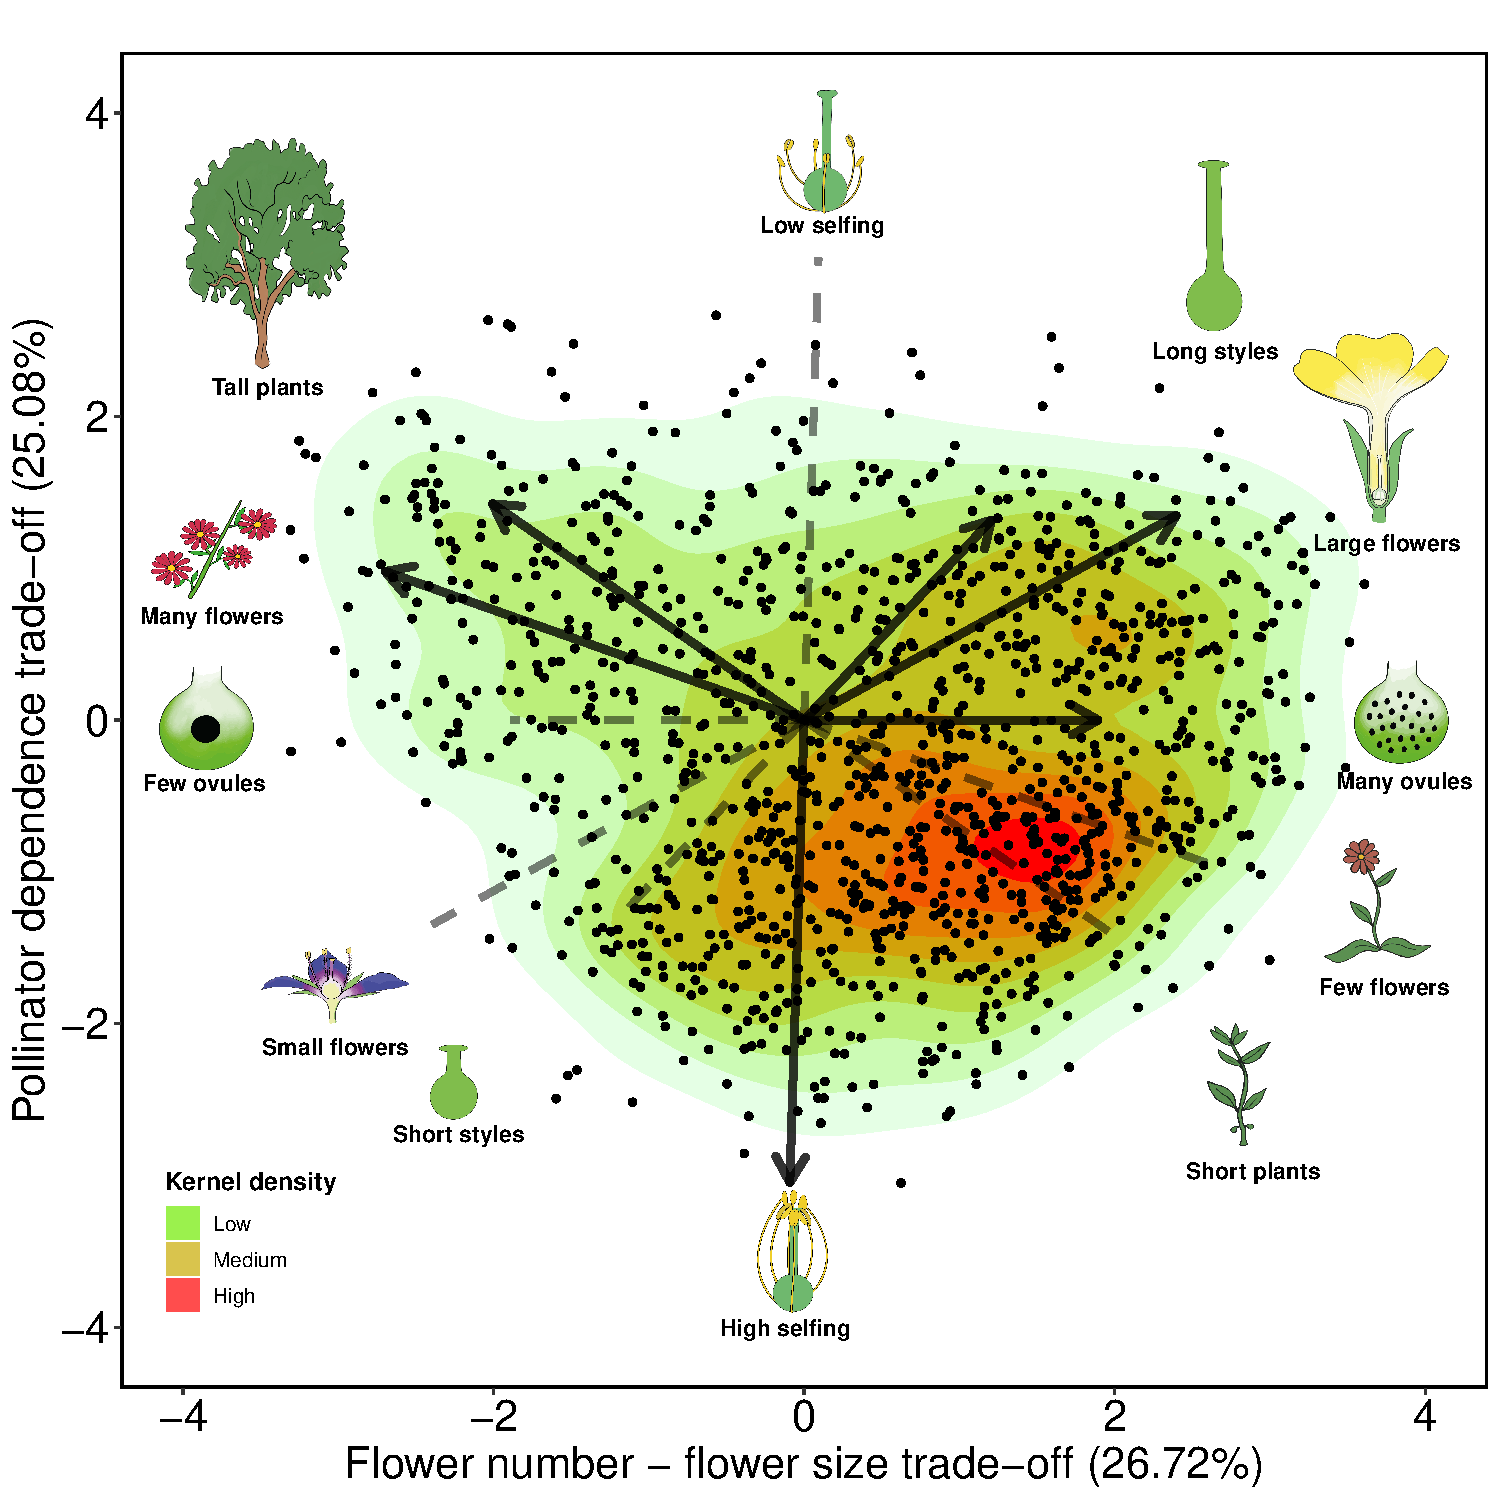
\includegraphics[width=0.95\linewidth]{output/figures/unnamed-chunk-2-1} 

}

\caption{\textbf{Figure 1} Phylogenetically informed principal component analysis (pPCA) of 1,236 plant species from 28 plant-pollinator network studies. The solid arrows indicate the direction of the different quantitative traits (flower number, plant height, style length, flower size, ovule number and level of autonomous selfing) across the two main axes of trait variation. The length of the arrows indicate the weight of the variables on each principal component and the dashed lines show the opposed direction of trait variation. The icons at both ends of arrows and dashed lines illustrate the extreme form of the trait continuum.}\label{fig:unnamed-chunk-2}
\end{figure}

We found (with an Anova) that most categorical traits were statistically associated with the first two axes of trait variation (Fig. 2 and Table S2). Flower symmetry, which was only associated with PC2 (Sum of squares = 8.51, F-value = 14.72, \emph{P} \textless{} 0.01 ), and nectar provision, which was independent of PC1 and PC2 (PC1: Sum of squares = 0.37, F-value = 0.29 , \emph{P} = 0.59; PC2: Sum of squares = 0.83, F-value = 1.43, \emph{P} = 0.23) showed lack of statistical association. In addition, we found (with a Tukey test) statistical differences between the different levels of categorical traits in the trait space (Fig. S8). Regarding self-compatibility, we found larger differences on PC2 (i.e., species with unisexual flowers that were self-incompatible were statistically differentiated from species with partial or full self-compatibility; Fig. S8a and Fig. S8b). Life forms differed statistically across both axes of trait variation and followed a gradient of larger life forms (trees and shrubs) with higher pollinator dependence to smaller ones (herbs) with lower pollinator dependence (Fig. S8c and Fig. S8d). Consequently, lifespan also followed this gradient but perennial and short lived species only differed statistically on PC2 (Fig. S8e and Fig. S8f). Species with unisexual flowers (monoecious and dioecious) were clustered on both extremes of the first two principal components and had the highest pollinator dependence and highest number of flowers (Fig. S8g and Fig. S8h). Moreover, we found that the campanulate and capitulum flower shapes were differentiated from tube, papilionaceous, open and brush shapes in the trait space. The former morphologies had larger flowers and greater pollinator dependence, while the latter had higher flower number and lower pollinator dependence (Fig. S8i and Fig. S8j). Regarding flower symmetry, zygomorphic flowers were associated with lower levels of pollinator dependence, whereas actinomorphic flowers had higher levels of pollinator dependence (Fig. S8k and Fig. S8l).

\blandscape

\begin{figure}[H]

{\centering 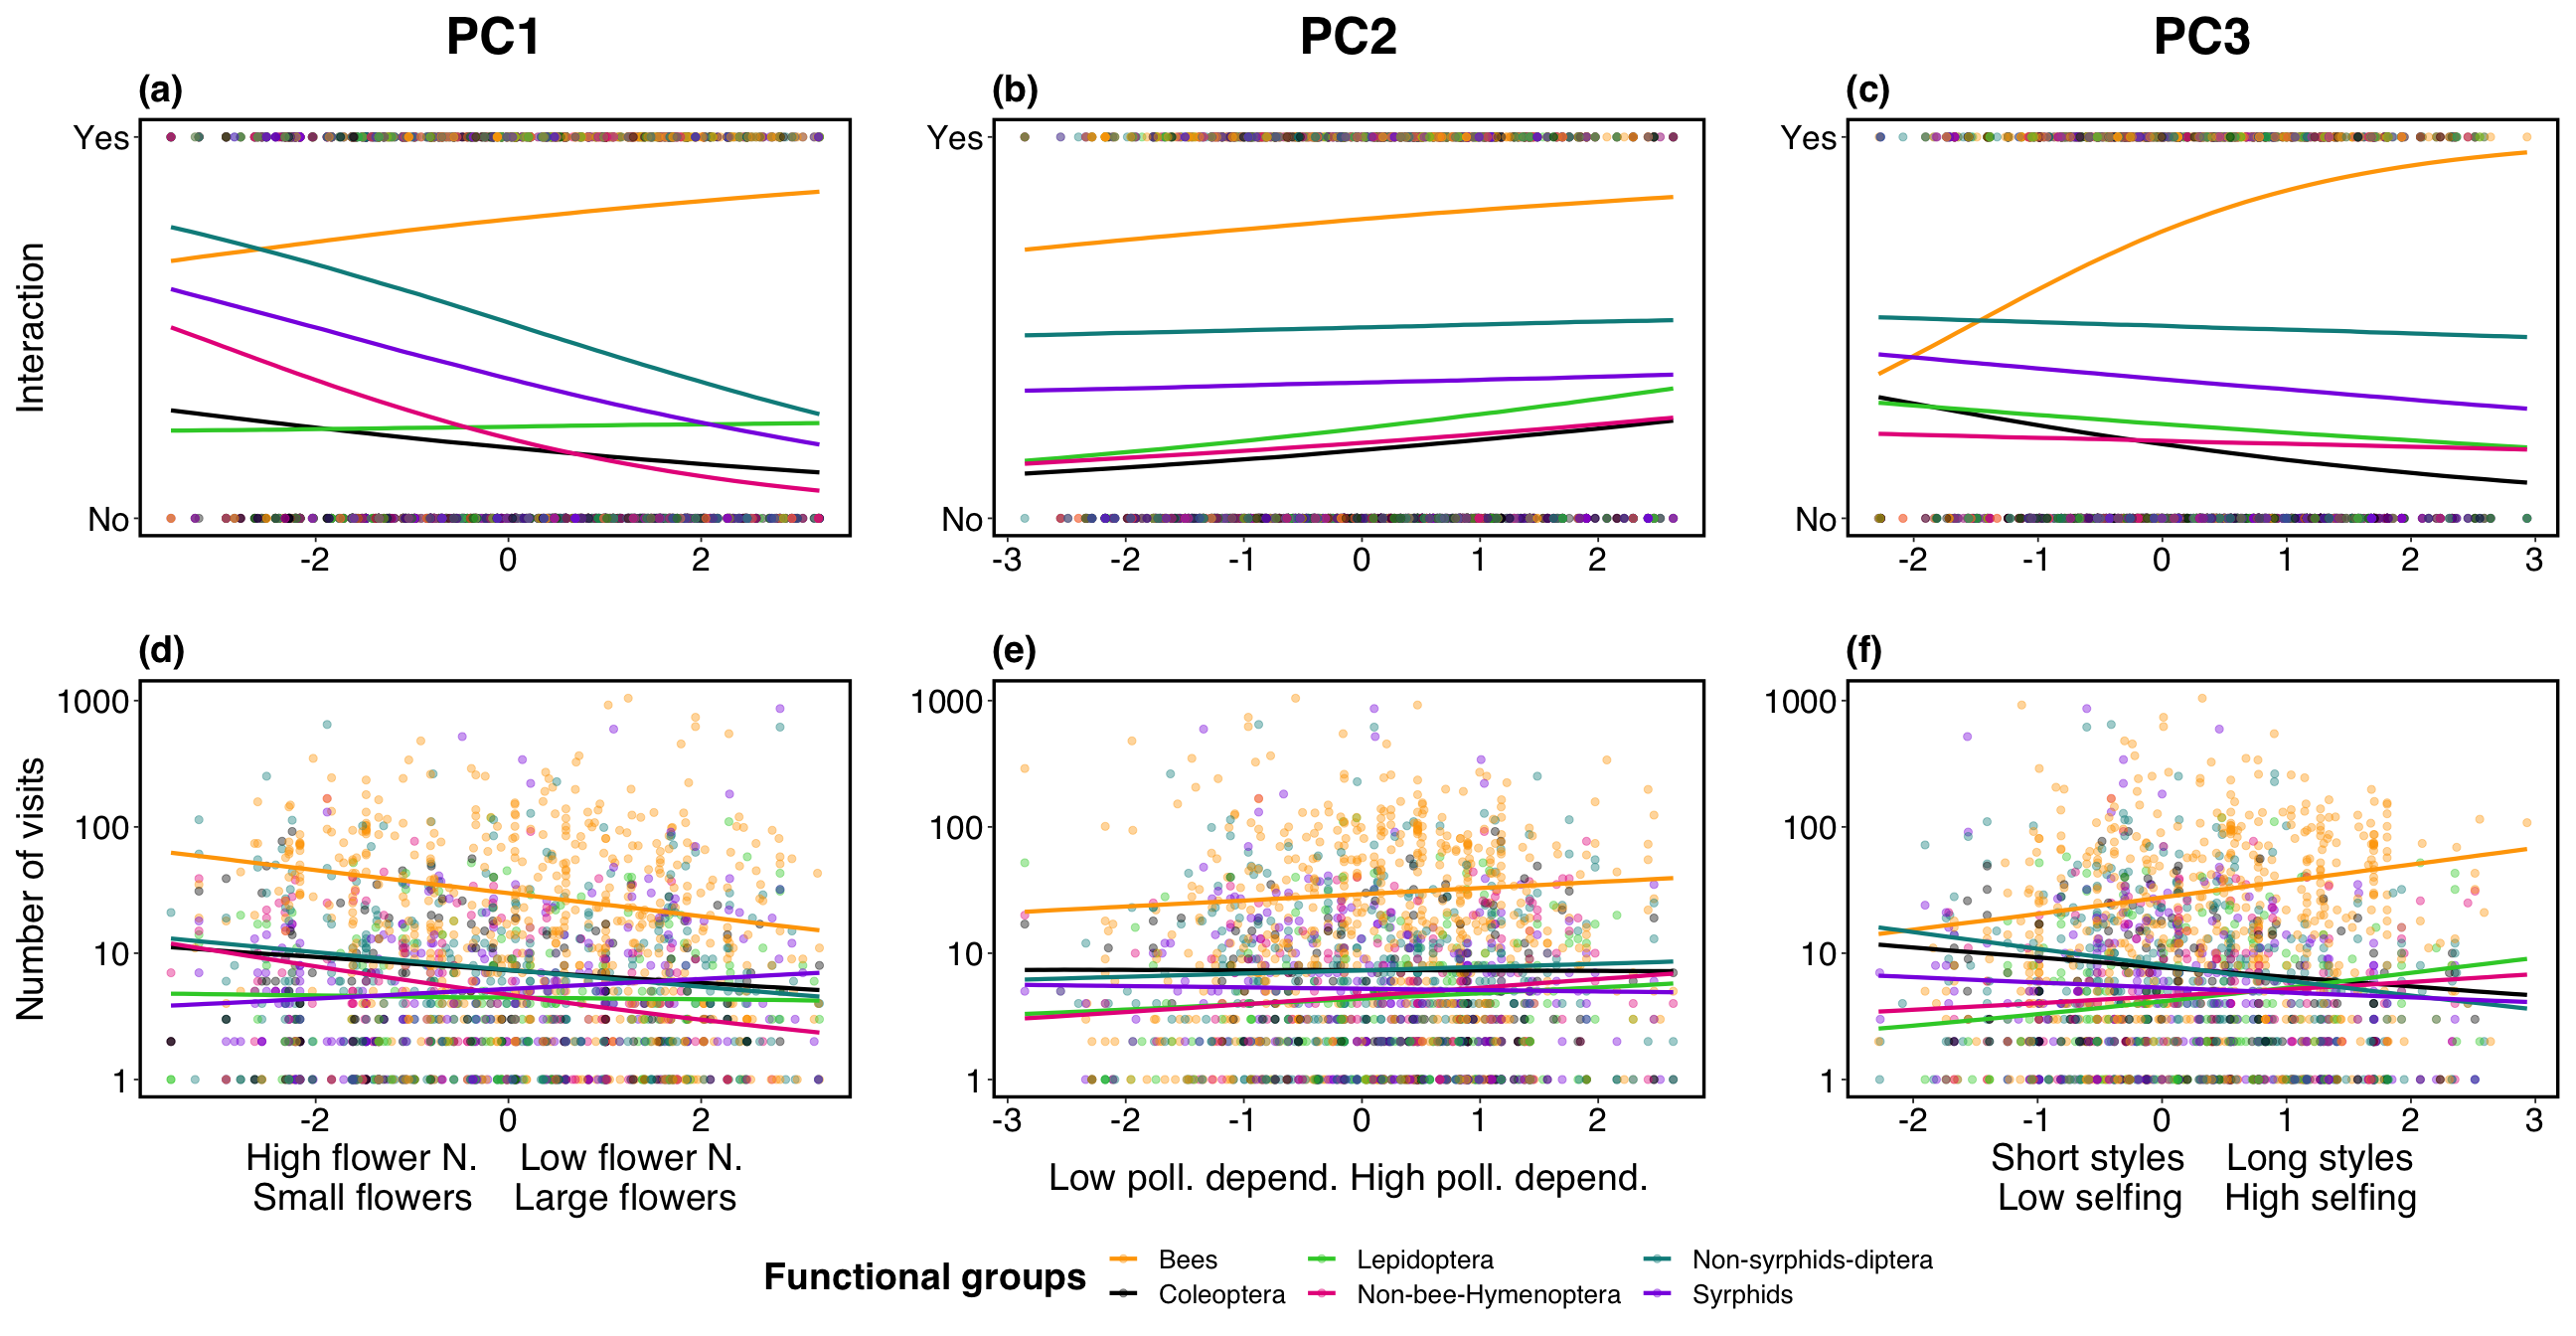
\includegraphics[width=0.8\linewidth]{output/figures/unnamed-chunk-3-1} 

}

\caption{\textbf{Figure 2} Location of the different qualitative traits on the trait space. The panel is composed by the traits that showed statistical association with the first two axes of trait variation: compatibility system (a), life form (b), lifespan (c), breeding system (d), flower shape (e) and flower symmetry (f). The solid arrows indicate the direction of variation of the different quantitative traits showed in figure 1: flower number (FN), plant height (PH), style length (SL), flower size (FS), ovule number (ON) and the level of autonomous selfing (S).}\label{fig:unnamed-chunk-3}
\end{figure}

\elandscape

\hypertarget{b-phylogenetic-signal}{%
\subsection{(b) Phylogenetic signal}\label{b-phylogenetic-signal}}

We found a strong phylogenetic signal (\emph{P} \textless{} 0.01) for most quantitative traits (Table S5). The traits that showed the highest phylogenetic signal were ovule number (\(\lambda\) = 1), pollen grains per flower (\(\lambda\) = 1) and plant height (\(\lambda\) = 0.96), followed by flower length (\(\lambda\) = 0.75), flower width (\(\lambda\) = 0.73), number of flowers per plant (\(\lambda\) = 0.69) and nectar concentration (\(\lambda\) = 0.65). The traits that showed a moderate phylogenetic signal were inflorescence width (\(\lambda\) = 0.57), style length (\(\lambda\) = 0.49) and autonomous selfing (\(\lambda\) = 0.34). Finally, microliters of nectar per flower showed the lowest phylogenetic signal of all traits (\(\lambda\) = 0.14).

\hypertarget{c-visitation-patterns}{%
\subsection{(c) Visitation patterns}\label{c-visitation-patterns}}

The main axes of trait variation (PC1, PC2 and PC3) explained partly presence-absence of interaction partners (conditional \(R^{2}\) = 0.26; marginal \(R^{2}\) = 0.20) but little of the overall number of visits (conditional \(R^{2}\) = 0.31; marginal \(R^{2}\) = 0.06). However, we found relevant differences across the different floral visitor guilds on both presence-absence of interactions and number of visits (Fig. 3). We found on the flower number - flower size axis that plants with high flower number and small flowers had higher interaction partners of Coleoptera, non-bee-Hymenoptera and all Diptera guilds (Fig. 3a) but plants with low flower number but large flowers had higher interaction partners of bees and Lepidoptera guilds. Regarding visitation rates on the flower number - flower size axis, we found similar trends but bees and syrphids guilds in this case showed higher number of visits to plant species with high flower number but small (Fig. 3d). On the pollinator dependence axis, we found that all plant species with higher pollinator dependence had higher number of interacting partners and number of visits from all floral visitor guilds (Fig. 3b and Fig. 3e). Finally, on the style length - pollinator dependence axis plant species with short styles and high pollinator dependence had higher interaction partners of all guilds but bees, that interacted clearly more with plant species with long styles and low pollinator dependence (Fig. 3c). However, regarding number of visits on the style length - pollinator dependence axis, we found that plants with long styles and high selfing interacted more frequently with Lepidoptera and non-bee-Hymenoptera guilds (Fig. 3f).

The additional model for both presence-absence of interaction (marginal \(R^{2}\) = 0.29; conditional \(R^{2}\) = 0.19) and number of visits (marginal \(R^{2}\) = 0.30; conditional \(R^{2}\) = 0.03) for the most represented families of bees showed that the family Apidae was the main driver of the observed patterns. The contrasting differences between presence-absence of interaction and number of visits for bees on PC1 (Fig. 3a and Fig. 3d) were driven by the family Andrenidae that had higher number of interacting partners but lower number of visits on plant species with low number of large flowers (Fig. S9).

\vspace{5mm}
\blandscape

\begin{figure}
\centering
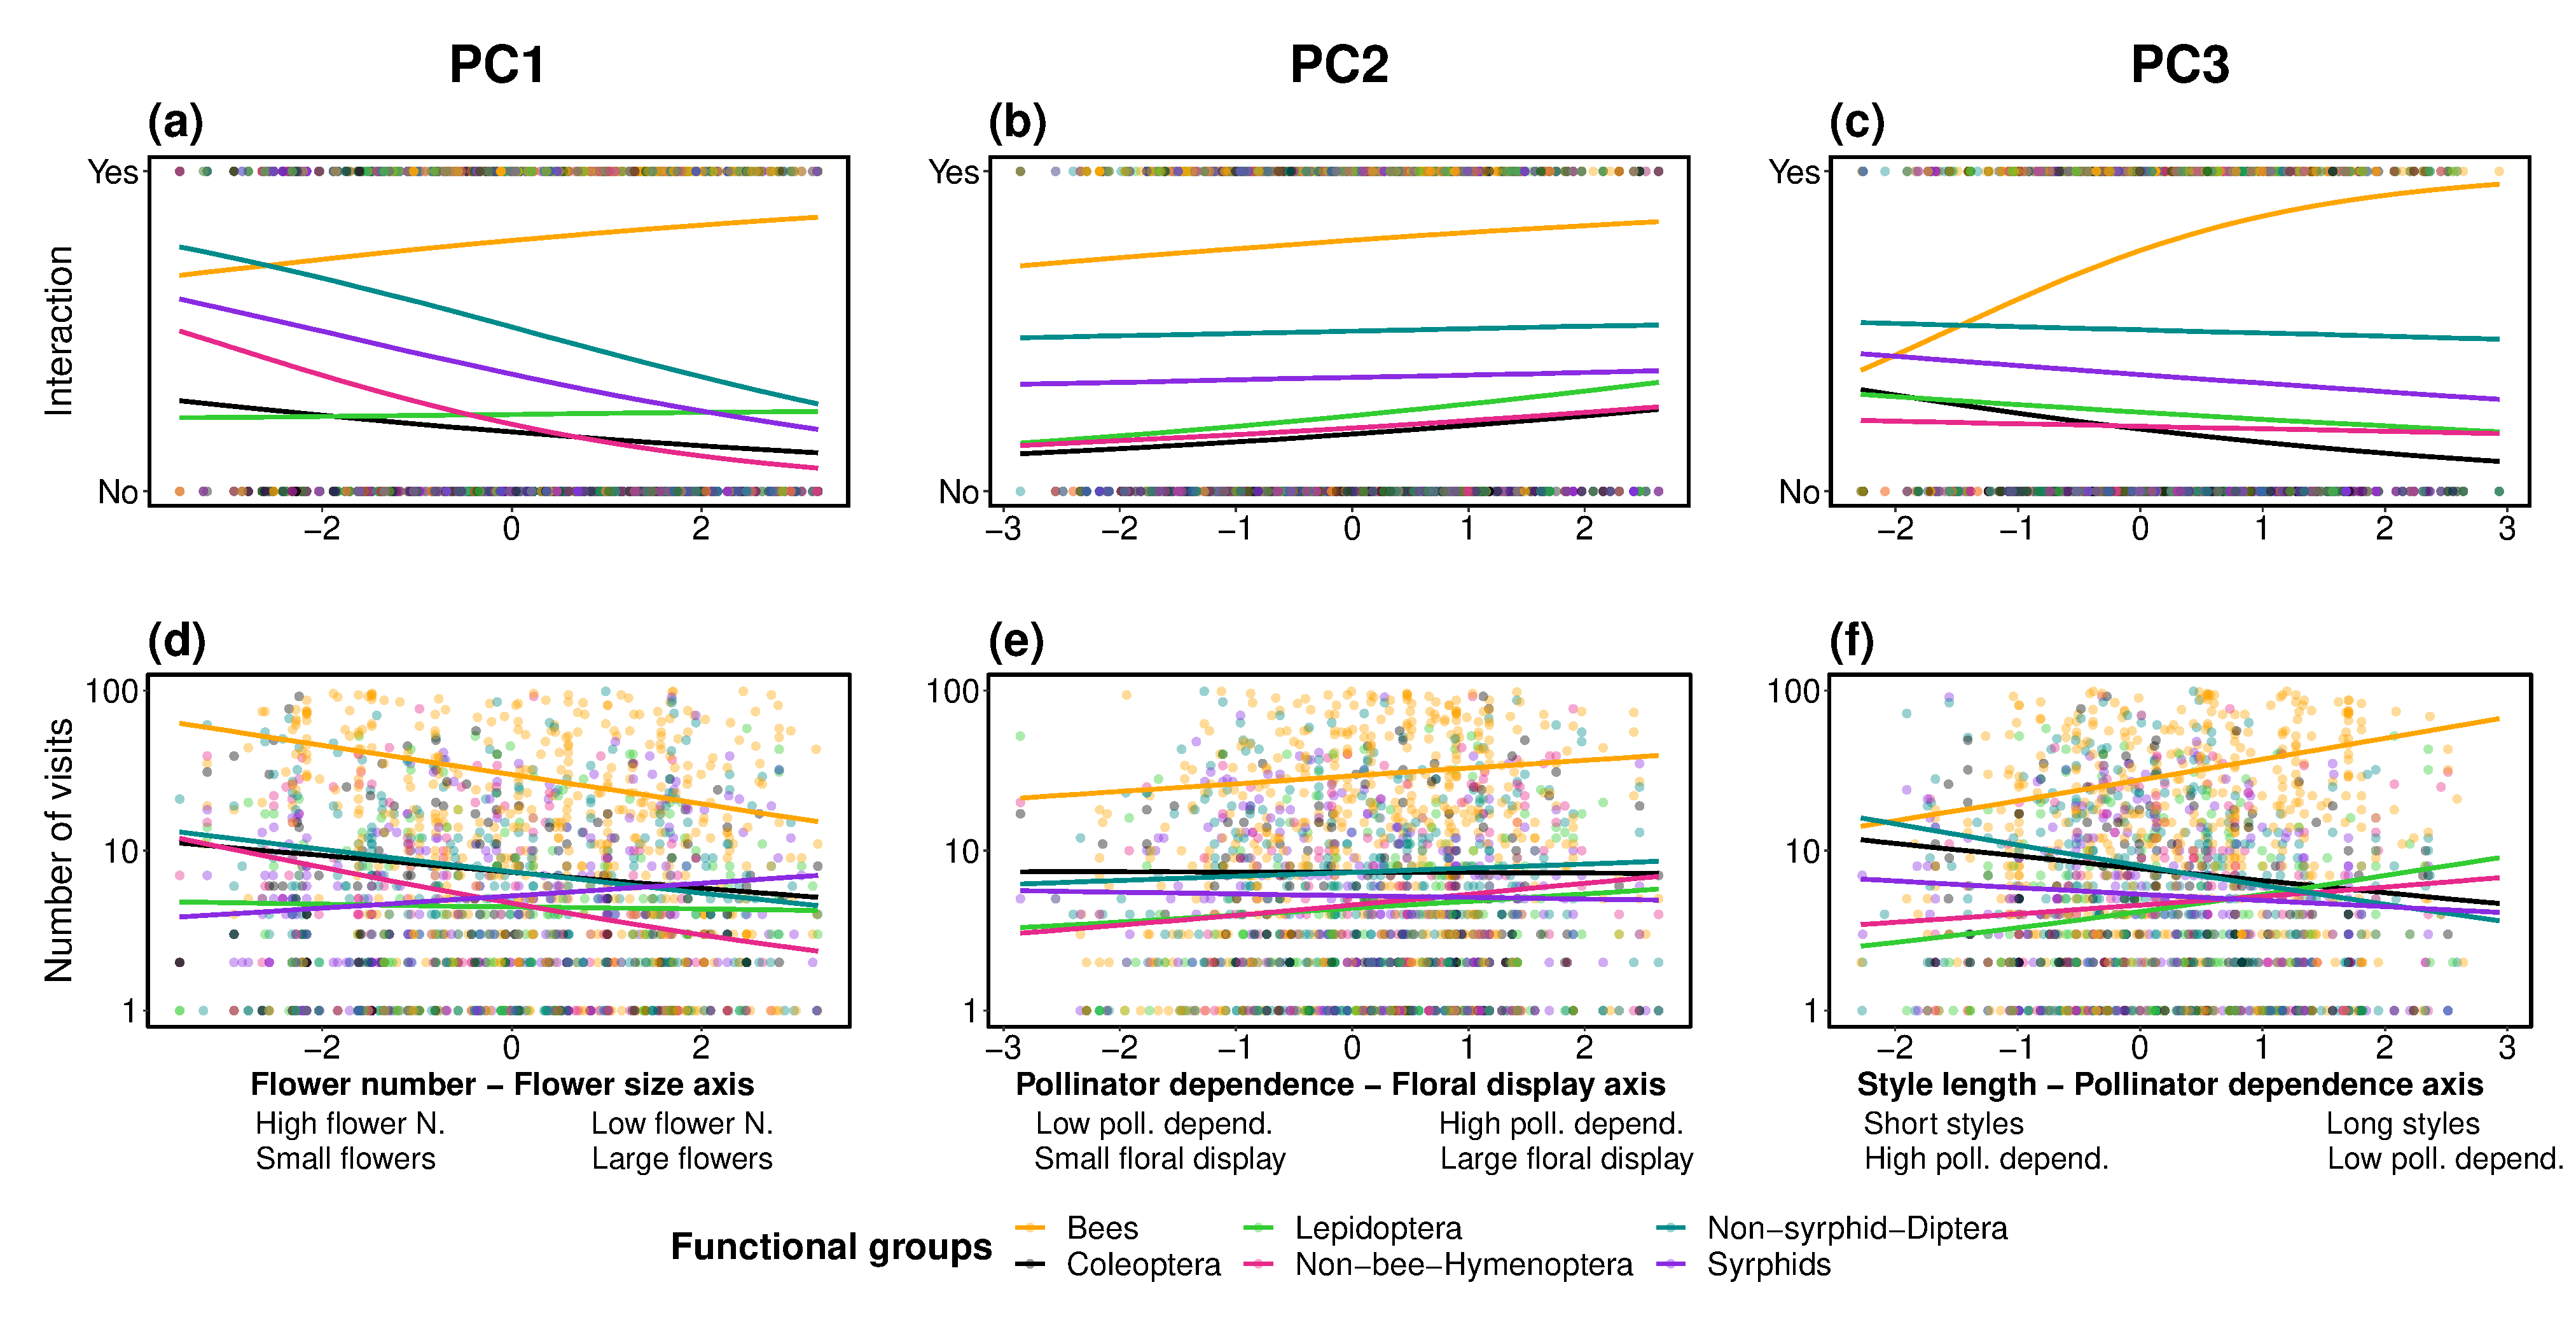
\includegraphics{output/figures/unnamed-chunk-4-1.pdf}
\caption{\label{fig:unnamed-chunk-4}\textbf{Figure 3} Fitted posterior estimates of the presence-absence of interaction (a, b and c) and number of visits (d, e and f) of the different floral visitor guilds in relation to the main axes of trait variation (PC1, PC2 and PC3). PC1 represents the flower number - flower size axis, PC2 represents the pollinator dependence axis and PC3, the style length - pollinator dependence axis. For visualization purposes, due to large differences between number of visits of bees and the rest of guilds, the number of visits was log-transformed (Y-axis of lower panel).}
\end{figure}

\elandscape

\hypertarget{d-plant-species-network-roles}{%
\subsection{(d) Plant species network roles}\label{d-plant-species-network-roles}}

The variance of the different plant species-level network metrics was poorly explained by the three main axes of trait variation (Fig. S10; number of visits \textasciitilde{} PCs, conditional \(R^{2}\) = 0.11, marginal \(R^{2}\) = 0.02; normalized degree \textasciitilde{} PCs, conditional \(R^{2}\) = 0.24, marginal \(R^{2}\) = 0.02; and, specialization \textasciitilde{} PCs, conditional \(R^{2}\) = 0.37, marginal\(R^{2}\) = 0.03). Overall, the most notable trends were found on the flower number - flower size axis (PC1) and the style length - pollinator dependence axis (PC3) for number of visits and specialization. On PC1, number of visits was higher for plant species with more flowers but was lower for plant species with larger flowers (Fig. S10a). However, specialization showed the opposite trend on this axis (Fig. S10g). On PC3, the number of visits was lower for plants with shorter styles and higher pollinator dependence but higher for plant species with longer styles and lower pollinator dependence (Fig. S10c). Again, specialization showed the opposite trend to number of visits (Fig. S10i).

\hypertarget{discussion}{%
\section{4. Discussion}\label{discussion}}

This study investigates the reproductive spectrum of flowering plants and shows that plants have clear positive and negative correlations between reproductive traits that determine interactions with floral visitors at a global scale. Despite the enormous variability of plant reproductive structures, the first two and three axes were able to capture over 50\% and 70\% of reproductive trait variation, respectively. These three axes were: (1) the flower number - flower size, (2) the pollinator dependence - floral display and (3) the style length - pollinator dependence. Although the explained trait variation that we found in the first two axes is lower than previous studies that consider only morphological and physiological traits {[}\protect\hyperlink{ref-diaz2016}{13},\protect\hyperlink{ref-carmona2021}{37}{]}, our results are consistent with the largest and most recent study that has characterised plant life strategies including reproductive and plant form and size related traits {[}\protect\hyperlink{ref-salguero2016}{7}{]}. Interestingly, these different plant reproductive axes were able to partly explain the number of interacting partners of floral visitor guilds. However, they were insufficient to capture their visitation rates which highlight the need to account for other factors to better capture the strength of these mutualistic interactions at a macroecological scale.

Our study provides solid evidence for several widely discussed trait associations with the help of a great diversity of phylogenetic lineages (170 families and over 1200 species) within a multitrait context. In addition, our work links the reproductive trait variation with the previously described fast-slow continuum' in plant {[}\protect\hyperlink{ref-salguero2016}{7}{]} and animal {[}\protect\hyperlink{ref-healy2019}{66}{]} life-history strategies, as indicated by the different floral and reproductive biology traits associated with plant height, life form and lifespan. Although the negative correlation between flower number and flower size has received substantial attention {[}\protect\hyperlink{ref-sargent2007}{39},\protect\hyperlink{ref-kettle2011}{40},\protect\hyperlink{ref-worley2000}{67}{]}, it has only been investigated across a few hundred of Angiosperm species with a two-trait approach. We found support to this trait association and show that other life history traits also covariate along this axis. For example, our study complements previous evidence that links breeding systems and life forms {[}\protect\hyperlink{ref-friedman2020}{8},\protect\hyperlink{ref-petit2006}{68}{]} by showing that most species with unisexual flowers are concentrated in the trait space and are associated with woody life forms with high flower number. Moreover, we also provide broad support for the previously documented positive association between outcrossing rate and floral display {[}\protect\hyperlink{ref-goodwillie2010}{41}{]} where species with high pollinator dependence have greater allocation of resources to attract floral visitors. Despite floral rewards not being included in the main analysis because there was insufficient data available, both pollen and nectar quantity were clearly associated with plant species with larger floral display. Thus, our results highlight the presence of worldwide reproductive trait covariation patterns across flowering plants that are likely to impose constraints to the global spectrum of plant trait variation.

Overall, our models showed that the main plant reproductive trait correlations have low predictive power for broad-level interaction patterns between plants and floral visitors. However, we found changes in the interaction patterns among and within floral visitor guilds that suggest that plant reproductive strategies partly mediate these associations at large ecological scales. For example, we found that all floral visitor guilds interacted more frequently with plant species with larger floral displays in agreement with previous findings {[}\protect\hyperlink{ref-lazaro2013}{28},\protect\hyperlink{ref-hegland2005}{69},\protect\hyperlink{ref-kaiser2014}{70}{]}. Because plants can adapt to the most efficient floral visitors {[}\protect\hyperlink{ref-fenster2004}{3}{]}, the different associations between specific set of traits and floral visitor guilds may indicate the existence of large scale pollination syndromes. For instance, bees and syrphid flies were clearly associated with opposing plant reproductive strategies and because these two guilds are likely to differ in ecology and behaviour {[}rader2020; {[}\protect\hyperlink{ref-foldesi2021}{71}{]}{]} they may exert different selective pressures that lead to divergent plant reproductive strategies. In any case, it is worth noting that other local factors such as species relative abundances, surely explain part of the observed variability {[}\protect\hyperlink{ref-bartomeus2016}{27},\protect\hyperlink{ref-vazquez2007}{72},\protect\hyperlink{ref-encinas2012}{73}{]} that reproductive correlations do not.

To conclude, we provide a robust description of the main reproductive trait covariation patterns of flowering plants by using a global dataset of plant reproductive traits from species that belong to plant-pollinator networks. Our work highlights the relevance of floral visitors in mediating these reproductive trait correlations and the need to consider other factors beyond plant reproductive strategies to better capture broad scale patterns of interactions with floral visitors. Our work provides empirical evidence that complements previous studies that have explored trait correlations with other plant organs and highlights the need to include these reproductive correlations in the global spectrum of plant form and function {[}\protect\hyperlink{ref-diaz2016}{13}{]} as reproductive strategies involve clear cost and benefits that can affect the trait space of the whole plant. Finally, the future incorporation of unrepresented areas of the world and other relevant reproductive traits such as flower life span or flower colour will definitely help to provide better descriptions of the reproductive spectrum of plant trait variation and plant-pollinator associations.

\hypertarget{references}{%
\section{References}\label{references}}

\hypertarget{refs}{}
\begin{CSLReferences}{0}{0}
\leavevmode\vadjust pre{\hypertarget{ref-barrett2002}{}}%
\CSLLeftMargin{1. }
\CSLRightInline{Barrett SCH. 2002 The evolution of plant sexual diversity. \emph{Nat. Rev. Genet.} \textbf{3}, 274--284. (doi:\href{https://doi.org/10.1038/nrg776}{10.1038/nrg776})}

\leavevmode\vadjust pre{\hypertarget{ref-schiestl2013}{}}%
\CSLLeftMargin{2. }
\CSLRightInline{Schiestl FP, Johnson SD. 2013 Pollinator-mediated evolution of floral signals. \emph{Trends Ecol. Evol.} \textbf{28}, 307--315. (doi:\href{https://doi.org/10.1016/j.tree.2013.01.019}{10.1016/j.tree.2013.01.019})}

\leavevmode\vadjust pre{\hypertarget{ref-fenster2004}{}}%
\CSLLeftMargin{3. }
\CSLRightInline{Fenster CB, Armbruster WS, Wilson P, Dudash MR, Thomson JD. 2004 Pollination {Syndromes} and {Floral Specialization}. \emph{Annu. Rev. Ecol. Evol. Syst.} \textbf{35}, 375--403. (doi:\href{https://doi.org/10.1146/annurev.ecolsys.34.011802.132347}{10.1146/annurev.ecolsys.34.011802.132347})}

\leavevmode\vadjust pre{\hypertarget{ref-dellinger2020}{}}%
\CSLLeftMargin{4. }
\CSLRightInline{Dellinger AS. 2020 Pollination syndromes in the 21st century: Where do we stand and where may we go? \emph{New Phytol.} \textbf{228}, 1193--1213. (doi:\href{https://doi.org/10.1111/nph.16793}{10.1111/nph.16793})}

\leavevmode\vadjust pre{\hypertarget{ref-stearns1989}{}}%
\CSLLeftMargin{5. }
\CSLRightInline{Stearns SC. 1989 Trade-offs in life-history evolution. \emph{Functional ecology} \textbf{3}, 259--268.}

\leavevmode\vadjust pre{\hypertarget{ref-agrawal2020}{}}%
\CSLLeftMargin{6. }
\CSLRightInline{Agrawal AA. 2020 A scale-dependent framework for trade-offs, syndromes, and specialization in organismal biology. \emph{Ecology} \textbf{101}, e02924.}

\leavevmode\vadjust pre{\hypertarget{ref-salguero2016}{}}%
\CSLLeftMargin{7. }
\CSLRightInline{Salguero-Gómez R, Jones OR, Jongejans E, Blomberg SP, Hodgson DJ, Mbeau-Ache C, Zuidema PA, de Kroon H, Buckley YM. 2016 Fast-slow continuum and reproductive strategies structure plant life-history variation worldwide. \emph{Proc. Natl. Acad. Sci. U.S.A.} \textbf{113}, 230--235. (doi:\href{https://doi.org/10.1073/pnas.1506215112}{10.1073/pnas.1506215112})}

\leavevmode\vadjust pre{\hypertarget{ref-friedman2020}{}}%
\CSLLeftMargin{8. }
\CSLRightInline{Friedman J. 2020 The evolution of annual and perennial plant life histories: Ecological correlates and genetic mechanisms. \emph{Annual Review of Ecology, Evolution, and Systematics} \textbf{51}, 461--481.}

\leavevmode\vadjust pre{\hypertarget{ref-paterno2020}{}}%
\CSLLeftMargin{9. }
\CSLRightInline{Paterno GB, Silveira CL, Kollmann J, Westoby M, Fonseca CR. 2020 The maleness of larger angiosperm flowers. \emph{Proceedings of the National Academy of Sciences} \textbf{117}, 10921--10926.}

\leavevmode\vadjust pre{\hypertarget{ref-roddy2021}{}}%
\CSLLeftMargin{10. }
\CSLRightInline{Roddy AB, Martínez-Perez C, Teixido AL, Cornelissen TG, Olson ME, Oliveira RS, Silveira FAO. 2021 Towards the flower economics spectrum. \emph{New Phytol.} \textbf{229}, 665--672. (doi:\href{https://doi.org/10.1111/nph.16823}{10.1111/nph.16823})}

\leavevmode\vadjust pre{\hypertarget{ref-wright2004}{}}%
\CSLLeftMargin{11. }
\CSLRightInline{Wright IJ \emph{et al.} 2004 The worldwide leaf economics spectrum. \emph{Nature} \textbf{428}, 821--827. (doi:\href{https://doi.org/10.1038/nature02403}{10.1038/nature02403})}

\leavevmode\vadjust pre{\hypertarget{ref-chave2009}{}}%
\CSLLeftMargin{12. }
\CSLRightInline{Chave J, Coomes D, Jansen S, Lewis SL, Swenson NG, Zanne AE. 2009 Towards a worldwide wood economics spectrum. \emph{Ecol. Lett.} \textbf{12}, 351--366.}

\leavevmode\vadjust pre{\hypertarget{ref-diaz2016}{}}%
\CSLLeftMargin{13. }
\CSLRightInline{Díaz S \emph{et al.} 2016 The global spectrum of plant form and function. \emph{Nature} \textbf{529}, 167--171. (doi:\href{https://doi.org/10.1038/nature16489}{10.1038/nature16489})}

\leavevmode\vadjust pre{\hypertarget{ref-onoda2017}{}}%
\CSLLeftMargin{14. }
\CSLRightInline{Onoda Y, Wright IJ, Evans JR, Hikosaka K, Kitajima K, Niinemets Ü, Poorter H, Tosens T, Westoby M. 2017 Physiological and structural tradeoffs underlying the leaf economics spectrum. \emph{New Phytologist} \textbf{214}, 1447--1463.}

\leavevmode\vadjust pre{\hypertarget{ref-laughlin2021}{}}%
\CSLLeftMargin{15. }
\CSLRightInline{Laughlin DC \emph{et al.} 2021 Root traits explain plant species distributions along climatic gradients yet challenge the nature of ecological trade-offs. \emph{Nat. Ecol. Evol.}, 1--12.}

\leavevmode\vadjust pre{\hypertarget{ref-baude2016}{}}%
\CSLLeftMargin{16. }
\CSLRightInline{Baude M, Kunin WE, Boatman ND, Conyers S, Davies N, Gillespie MA, Morton RD, Smart SM, Memmott J. 2016 Historical nectar assessment reveals the fall and rise of floral resources in britain. \emph{Nature} \textbf{530}, 85--88.}

\leavevmode\vadjust pre{\hypertarget{ref-munoz2016}{}}%
\CSLLeftMargin{17. }
\CSLRightInline{Munoz F, Violle C, Cheptou P-O. 2016 {CSR} ecological strategies and plant mating systems: Outcrossing increases with competitiveness but stress-tolerance is related to mixed mating. \emph{Oikos} \textbf{125}, 1296--1303. (doi:\href{https://doi.org/10.1111/oik.02328}{10.1111/oik.02328})}

\leavevmode\vadjust pre{\hypertarget{ref-grossenbacher2017}{}}%
\CSLLeftMargin{18. }
\CSLRightInline{Grossenbacher DL \emph{et al.} 2017 Self-compatibility is over-represented on islands. \emph{New Phytol.} \textbf{215}, 469--478.}

\leavevmode\vadjust pre{\hypertarget{ref-moeller2017}{}}%
\CSLLeftMargin{19. }
\CSLRightInline{Moeller DA \emph{et al.} 2017 Global biogeography of mating system variation in seed plants. \emph{Ecol. Lett.} \textbf{20}, 375--384. (doi:\href{https://doi.org/10.1111/ele.12738}{10.1111/ele.12738})}

\leavevmode\vadjust pre{\hypertarget{ref-sargent2008}{}}%
\CSLLeftMargin{20. }
\CSLRightInline{Sargent RD, Ackerly DD. 2008 Plant--pollinator interactions and the assembly of plant communities. \emph{Trends Ecol. Evol.} \textbf{23}, 123--130.}

\leavevmode\vadjust pre{\hypertarget{ref-rech2016}{}}%
\CSLLeftMargin{21. }
\CSLRightInline{Rech AR, Dalsgaard B, Sandel B, Sonne J, Svenning J-C, Holmes N, Ollerton J. 2016 The macroecology of animal versus wind pollination: Ecological factors are more important than historical climate stability. \emph{Plant Ecol. Divers.} \textbf{9}, 253--262. (doi:\href{https://doi.org/10.1080/17550874.2016.1207722}{10.1080/17550874.2016.1207722})}

\leavevmode\vadjust pre{\hypertarget{ref-ruger2018}{}}%
\CSLLeftMargin{22. }
\CSLRightInline{Rüger N, Comita LS, Condit R, Purves D, Rosenbaum B, Visser MD, Wright SJ, Wirth C. 2018 Beyond the fast\textendash slow continuum: Demographic dimensions structuring a tropical tree community. \emph{Ecol. Lett.} \textbf{21}, 1075--1084. (doi:\href{https://doi.org/10.1111/ele.12974}{10.1111/ele.12974})}

\leavevmode\vadjust pre{\hypertarget{ref-tur2013}{}}%
\CSLLeftMargin{23. }
\CSLRightInline{Tur C, Castro-Urgal R, Traveset A. 2013 Linking {Plant Specialization} to {Dependence} in {Interactions} for {Seed Set} in {Pollination Networks}. \emph{PLoS One} \textbf{8}, e78294. (doi:\href{https://doi.org/10.1371/journal.pone.0078294}{10.1371/journal.pone.0078294})}

\leavevmode\vadjust pre{\hypertarget{ref-devaux2014}{}}%
\CSLLeftMargin{24. }
\CSLRightInline{Devaux C, Lepers C, Porcher E. 2014 Constraints imposed by pollinator behaviour on the ecology and evolution of plant mating systems. \emph{J. Evol. Biol.} \textbf{27}, 1413--1430. (doi:\href{https://doi.org/10.1111/jeb.12380}{10.1111/jeb.12380})}

\leavevmode\vadjust pre{\hypertarget{ref-rosas2014}{}}%
\CSLLeftMargin{25. }
\CSLRightInline{Rosas-Guerrero V, Aguilar R, Martén-Rodríguez S, Ashworth L, Lopezaraiza-Mikel M, Bastida JM, Quesada M. 2014 A quantitative review of pollination syndromes: Do floral traits predict effective pollinators? \emph{Ecol. Lett.} \textbf{17}, 388--400.}

\leavevmode\vadjust pre{\hypertarget{ref-stang2009}{}}%
\CSLLeftMargin{26. }
\CSLRightInline{Stang M, Klinkhamer PGL, Waser NM, Stang I, van der Meijden E. 2009 Size-specific interaction patterns and size matching in a plant\textendash pollinator interaction web. \emph{Ann. Bot.} \textbf{103}, 1459--1469. (doi:\href{https://doi.org/10.1093/aob/mcp027}{10.1093/aob/mcp027})}

\leavevmode\vadjust pre{\hypertarget{ref-bartomeus2016}{}}%
\CSLLeftMargin{27. }
\CSLRightInline{Bartomeus I, Gravel D, Tylianakis JM, Aizen MA, Dickie IA, Bernard-Verdier M. 2016 A common framework for identifying linkage rules across different types of interactions. \emph{Funct. Ecol.} \textbf{30}, 1894--1903. (doi:\href{https://doi.org/10.1111/1365-2435.12666}{10.1111/1365-2435.12666})}

\leavevmode\vadjust pre{\hypertarget{ref-lazaro2013}{}}%
\CSLLeftMargin{28. }
\CSLRightInline{Lázaro A, Jakobsson A, Totland Ø. 2013 How do pollinator visitation rate and seed set relate to species' floral traits and community context? \emph{Oecologia} \textbf{173}, 881--893. (doi:\href{https://doi.org/10.1007/s00442-013-2652-5}{10.1007/s00442-013-2652-5})}

\leavevmode\vadjust pre{\hypertarget{ref-junker2013}{}}%
\CSLLeftMargin{29. }
\CSLRightInline{Junker RR, Blüthgen N, Brehm T, Binkenstein J, Paulus J, Schaefer HM, Stang M. 2013 Specialization on traits as basis for the niche-breadth of flower visitors and as structuring mechanism of ecological networks. \emph{Funct. Ecol.} \textbf{27}, 329--341. (doi:\href{https://doi.org/10.1111/1365-2435.12005}{10.1111/1365-2435.12005})}

\leavevmode\vadjust pre{\hypertarget{ref-coux2016}{}}%
\CSLLeftMargin{30. }
\CSLRightInline{Coux C, Rader R, Bartomeus I, Tylianakis JM. 2016 Linking species functional roles to their network roles. \emph{Ecol. Lett.} \textbf{19}, 762--770. (doi:\href{https://doi.org/10.1111/ele.12612}{10.1111/ele.12612})}

\leavevmode\vadjust pre{\hypertarget{ref-ibanez2012}{}}%
\CSLLeftMargin{31. }
\CSLRightInline{Ibanez S. 2012 Optimizing size thresholds in a plant-pollinator interaction web: Towards a mechanistic understanding of ecological networks. \emph{Oecologia} \textbf{170}, 233--242. (doi:\href{https://doi.org/10.1007/s00442-012-2290-3}{10.1007/s00442-012-2290-3})}

\leavevmode\vadjust pre{\hypertarget{ref-eklof2013}{}}%
\CSLLeftMargin{32. }
\CSLRightInline{Eklöf A \emph{et al.} 2013 The dimensionality of ecological networks. \emph{Ecol. Lett.} \textbf{16}, 577--583.}

\leavevmode\vadjust pre{\hypertarget{ref-dehling2016}{}}%
\CSLLeftMargin{33. }
\CSLRightInline{Dehling DM, Jordano P, Schaefer HM, Böhning-Gaese K, Schleuning M. 2016 Morphology predicts species' functional roles and their degree of specialization in plant--frugivore interactions. \emph{Proc. Royal Soc. B} \textbf{283}, 20152444.}

\leavevmode\vadjust pre{\hypertarget{ref-kattge2011}{}}%
\CSLLeftMargin{34. }
\CSLRightInline{Kattge J \emph{et al.} 2011 {TRY} \textendash{} a global database of plant traits. \emph{Glob. Chang. Biol.} \textbf{17}, 2905--2935. (doi:\href{https://doi.org/10.1111/j.1365-2486.2011.02451.x}{10.1111/j.1365-2486.2011.02451.x})}

\leavevmode\vadjust pre{\hypertarget{ref-salguero2015}{}}%
\CSLLeftMargin{35. }
\CSLRightInline{Salguero-Gómez R \emph{et al.} 2015 The compadre {Plant Matrix Database}: An open online repository for plant demography. \emph{J. Ecol.} \textbf{103}, 202--218. (doi:\href{https://doi.org/10.1111/1365-2745.12334}{10.1111/1365-2745.12334})}

\leavevmode\vadjust pre{\hypertarget{ref-bruelheide2018}{}}%
\CSLLeftMargin{36. }
\CSLRightInline{Bruelheide H \emph{et al.} 2018 Global trait--environment relationships of plant communities. \emph{Nat. Ecol. Evol.} \textbf{2}, 1906--1917.}

\leavevmode\vadjust pre{\hypertarget{ref-carmona2021}{}}%
\CSLLeftMargin{37. }
\CSLRightInline{Carmona CP \emph{et al.} 2021 Erosion of global functional diversity across the tree of life. \emph{Sci. Adv.} \textbf{7}, eabf2675. (doi:\href{https://doi.org/10.1126/sciadv.abf2675}{10.1126/sciadv.abf2675})}

\leavevmode\vadjust pre{\hypertarget{ref-evojtko2020}{}}%
\CSLLeftMargin{38. }
\CSLRightInline{E-Vojtkó A, Bello F de, Durka W, Kühn I, Götzenberger L. 2020 The neglected importance of floral traits in trait-based plant community assembly. \emph{J. Veg. Sci.} \textbf{31}, 529--539. (doi:\href{https://doi.org/10.1111/jvs.12877}{10.1111/jvs.12877})}

\leavevmode\vadjust pre{\hypertarget{ref-sargent2007}{}}%
\CSLLeftMargin{39. }
\CSLRightInline{Sargent RD, Goodwillie C, Kalisz S, Ree RH. 2007 Phylogenetic evidence for a flower size and number trade-off. \emph{Am. J. Bot.} \textbf{94}, 2059--2062. (doi:\href{https://doi.org/10.3732/ajb.94.12.2059}{10.3732/ajb.94.12.2059})}

\leavevmode\vadjust pre{\hypertarget{ref-kettle2011}{}}%
\CSLLeftMargin{40. }
\CSLRightInline{Kettle CJ, Maycock CR, Ghazoul J, Hollingsworth PM, Khoo E, Sukri RSH, Burslem DFRP. 2011 Ecological {Implications} of a {Flower Size}/{Number Trade}-{Off} in {Tropical Forest Trees}. \emph{PLoS One} \textbf{6}, e16111. (doi:\href{https://doi.org/10.1371/journal.pone.0016111}{10.1371/journal.pone.0016111})}

\leavevmode\vadjust pre{\hypertarget{ref-goodwillie2010}{}}%
\CSLLeftMargin{41. }
\CSLRightInline{Goodwillie C \emph{et al.} 2010 Correlated evolution of mating system and floral display traits in flowering plants and its implications for the distribution of mating system variation. \emph{New Phytol.} \textbf{185}, 311--321. (doi:\href{https://doi.org/10.1111/j.1469-8137.2009.03043.x}{10.1111/j.1469-8137.2009.03043.x})}

\leavevmode\vadjust pre{\hypertarget{ref-barrett2003}{}}%
\CSLLeftMargin{42. }
\CSLRightInline{Barrett SCH. 2003 Mating strategies in flowering plants: The outcrossing-selfing paradigm and beyond. \emph{Philos. Trans. R. Soc. Lond. B Biol. Sci.} \textbf{358}, 991--1004. (doi:\href{https://doi.org/10.1098/rstb.2003.1301}{10.1098/rstb.2003.1301})}

\leavevmode\vadjust pre{\hypertarget{ref-carvalheiro2014}{}}%
\CSLLeftMargin{43. }
\CSLRightInline{Carvalheiro LG \emph{et al.} 2014 The potential for indirect effects between co-flowering plants via shared pollinators depends on resource abundance, accessibility and relatedness. \emph{Ecol. Lett.} \textbf{17}, 1389--1399. (doi:\href{https://doi.org/10.1111/ele.12342}{10.1111/ele.12342})}

\leavevmode\vadjust pre{\hypertarget{ref-olesen2007}{}}%
\CSLLeftMargin{44. }
\CSLRightInline{Olesen JM, Bascompte J, Dupont YL, Jordano P. 2007 The modularity of pollination networks. \emph{PNAS} \textbf{104}, 19891--19896. (doi:\href{https://doi.org/10.1073/pnas.0706375104}{10.1073/pnas.0706375104})}

\leavevmode\vadjust pre{\hypertarget{ref-fortuna2010}{}}%
\CSLLeftMargin{45. }
\CSLRightInline{Fortuna MA, Stouffer DB, Olesen JM, Jordano P, Mouillot D, Krasnov BR, Poulin R, Bascompte J. 2010 Nestedness versus modularity in ecological networks: Two sides of the same coin? \emph{J. Anim. Ecol.} \textbf{79}, 811--817. (doi:\href{https://doi.org/10.1111/j.1365-2656.2010.01688.x}{10.1111/j.1365-2656.2010.01688.x})}

\leavevmode\vadjust pre{\hypertarget{ref-poisot2016}{}}%
\CSLLeftMargin{46. }
\CSLRightInline{Poisot T \emph{et al.} 2016 Mangal \textendash{} making ecological network analysis simple. \emph{Ecography} \textbf{39}, 384--390. (doi:\href{https://doi.org/10.1111/ecog.00976}{10.1111/ecog.00976})}

\leavevmode\vadjust pre{\hypertarget{ref-chamberlain2020}{}}%
\CSLLeftMargin{47. }
\CSLRightInline{Chamberlain S \emph{et al.} 2020 Taxize: {Taxonomic} information from around the web. R package version 0.9.99.~At \href{https://CRAN.R-project.org/package=taxize}{https://CRAN.r-project.org/package=taxize}. }

\leavevmode\vadjust pre{\hypertarget{ref-smith2018}{}}%
\CSLLeftMargin{48. }
\CSLRightInline{Smith SA, Brown JW. 2018 Constructing a broadly inclusive seed plant phylogeny. \emph{Am. J. Bot.} \textbf{105}, 302--314. (doi:\href{https://doi.org/10.1002/ajb2.1019}{10.1002/ajb2.1019})}

\leavevmode\vadjust pre{\hypertarget{ref-jin2019}{}}%
\CSLLeftMargin{49. }
\CSLRightInline{Jin Y, Qian H. 2019 V.{PhyloMaker}: An {R} package that can generate very large phylogenies for vascular plants. \emph{Ecography} \textbf{42}, 1353--1359. (doi:\href{https://doi.org/10.1111/ecog.04434}{10.1111/ecog.04434})}

\leavevmode\vadjust pre{\hypertarget{ref-stekhoven2012}{}}%
\CSLLeftMargin{50. }
\CSLRightInline{Stekhoven DJ, Bühlmann P. 2012 {MissForest}\textemdash non-parametric missing value imputation for mixed-type data. \emph{Bioinformatics} \textbf{28}, 112--118. (doi:\href{https://doi.org/10.1093/bioinformatics/btr597}{10.1093/bioinformatics/btr597})}

\leavevmode\vadjust pre{\hypertarget{ref-penone2014}{}}%
\CSLLeftMargin{51. }
\CSLRightInline{Penone C, Davidson AD, Shoemaker KT, Marco MD, Rondinini C, Brooks TM, Young BE, Graham CH, Costa GC. 2014 Imputation of missing data in life-history trait datasets: Which approach performs the best? \emph{Methods Ecol. Evol.} \textbf{5}, 961--970. (doi:\href{https://doi.org/10.1111/2041-210X.12232}{10.1111/2041-210X.12232})}

\leavevmode\vadjust pre{\hypertarget{ref-santos2018}{}}%
\CSLLeftMargin{52. }
\CSLRightInline{Chamberlain S \emph{et al.} 2018 Package {``{PVR}''}. R package version 0.3.~At \href{https://CRAN.R-project.org/package=PVR}{https://CRAN.r-project.org/package=PVR}. }

\leavevmode\vadjust pre{\hypertarget{ref-diniz-filho2012}{}}%
\CSLLeftMargin{53. }
\CSLRightInline{Diniz-Filho JAF, Bini LM, Rangel TF, Morales-Castilla I, Olalla-Tárraga MÁ, Rodríguez MÁ, Hawkins BA. 2012 On the selection of phylogenetic eigenvectors for ecological analyses. \emph{Ecography} \textbf{35}, 239--249. (doi:\href{https://doi.org/10.1111/j.1600-0587.2011.06949.x}{10.1111/j.1600-0587.2011.06949.x})}

\leavevmode\vadjust pre{\hypertarget{ref-serneels2008}{}}%
\CSLLeftMargin{54. }
\CSLRightInline{Serneels S, Verdonck T. 2008 Principal component analysis for data containing outliers and missing elements. \emph{Computational Statistics \& Data Analysis} \textbf{52}, 1712--1727.}

\leavevmode\vadjust pre{\hypertarget{ref-legendre2012}{}}%
\CSLLeftMargin{55. }
\CSLRightInline{Legendre P, Legendre L. 2012 \emph{Numerical ecology}. {2nd edn}. {Elsevier, Amsterdam}. }

\leavevmode\vadjust pre{\hypertarget{ref-revell2012}{}}%
\CSLLeftMargin{56. }
\CSLRightInline{Revell LJ. 2012 Phytools: An {R} package for phylogenetic comparative biology (and other things). \emph{Methods Ecol. Evol.} \textbf{3}, 217--223. (doi:\href{https://doi.org/10.1111/j.2041-210X.2011.00169.x}{10.1111/j.2041-210X.2011.00169.x})}

\leavevmode\vadjust pre{\hypertarget{ref-abdi2010}{}}%
\CSLLeftMargin{57. }
\CSLRightInline{Abdi H, Williams LJ. 2010 Principal component analysis. \emph{WIREs Comp. Stats.} \textbf{2}, 433--459. (doi:\href{https://doi.org/10.1002/wics.101}{10.1002/wics.101})}

\leavevmode\vadjust pre{\hypertarget{ref-ballantyne2015}{}}%
\CSLLeftMargin{58. }
\CSLRightInline{Ballantyne G, Baldock KCR, Willmer PG. 2015 Constructing more informative plant\textendash pollinator networks: Visitation and pollen deposition networks in a heathland plant community. \emph{Proc. Royal Soc. B} \textbf{282}, 20151130. (doi:\href{https://doi.org/10.1098/rspb.2015.1130}{10.1098/rspb.2015.1130})}

\leavevmode\vadjust pre{\hypertarget{ref-vazquez2005}{}}%
\CSLLeftMargin{59. }
\CSLRightInline{Vázquez DP, Morris WF, Jordano P. 2005 Interaction frequency as a surrogate for the total effect of animal mutualists on plants. \emph{Ecol. Lett.} \textbf{8}, 1088--1094. (doi:\href{https://doi.org/10.1111/j.1461-0248.2005.00810.x}{10.1111/j.1461-0248.2005.00810.x})}

\leavevmode\vadjust pre{\hypertarget{ref-vazquez2012}{}}%
\CSLLeftMargin{60. }
\CSLRightInline{Vázquez DP, Lomáscolo SB, Maldonado MB, Chacoff NP, Dorado J, Stevani EL, Vitale NL. 2012 The strength of plant\textendash pollinator interactions. \emph{Ecology} \textbf{93}, 719--725. (doi:\href{https://doi.org/10.1890/11-1356.1}{10.1890/11-1356.1})}

\leavevmode\vadjust pre{\hypertarget{ref-hung2018}{}}%
\CSLLeftMargin{61. }
\CSLRightInline{Hung K-LJ, Kingston JM, Albrecht M, Holway DA, Kohn JR. 2018 The worldwide importance of honey bees as pollinators in natural habitats. \emph{Proc. Royal Soc. B} \textbf{285}, 20172140.}

\leavevmode\vadjust pre{\hypertarget{ref-burkner2017}{}}%
\CSLLeftMargin{62. }
\CSLRightInline{Bürkner P-C. 2017 Brms: {An R} package for {Bayesian} multilevel models using {Stan}. \emph{J. Stat. Softw.} \textbf{80}, 1--28.}

\leavevmode\vadjust pre{\hypertarget{ref-gabry2019}{}}%
\CSLLeftMargin{63. }
\CSLRightInline{Gabry J, Simpson D, Vehtari A, Betancourt M, Gelman A. 2019 Visualization in {Bayesian} workflow. \emph{J. R. Stat. Soc. Ser. A Stat. Soc.} \textbf{182}, 389--402. (doi:\href{https://doi.org/10.1111/rssa.12378}{10.1111/rssa.12378})}

\leavevmode\vadjust pre{\hypertarget{ref-dormann2008}{}}%
\CSLLeftMargin{64. }
\CSLRightInline{Dormann CF, Gruber B, Fründ J. 2008 Introducing the bipartite package: Analysing ecological networks. \emph{R News} \textbf{8/2}.}

\leavevmode\vadjust pre{\hypertarget{ref-bluthgen2006}{}}%
\CSLLeftMargin{65. }
\CSLRightInline{Blüthgen N, Menzel F, Blüthgen N. 2006 Measuring specialization in species interaction networks. \emph{BMC Ecol.} \textbf{6}, 9. (doi:\href{https://doi.org/10.1186/1472-6785-6-9}{10.1186/1472-6785-6-9})}

\leavevmode\vadjust pre{\hypertarget{ref-healy2019}{}}%
\CSLLeftMargin{66. }
\CSLRightInline{Healy K, Ezard THG, Jones OR, Salguero-Gómez R, Buckley YM. 2019 Animal life history is shaped by the pace of life and the distribution of age-specific mortality and reproduction. \emph{Nat. Ecol. Evol.} \textbf{3}, 1217--1224. (doi:\href{https://doi.org/10.1038/s41559-019-0938-7}{10.1038/s41559-019-0938-7})}

\leavevmode\vadjust pre{\hypertarget{ref-worley2000}{}}%
\CSLLeftMargin{67. }
\CSLRightInline{Worley AC, Baker AM, Thompson JD, Barrett SC. 2000 Floral display in narcissus: Variation in flower size and number at the species, population, and individual levels. \emph{International Journal of Plant Sciences} \textbf{161}, 69--79.}

\leavevmode\vadjust pre{\hypertarget{ref-petit2006}{}}%
\CSLLeftMargin{68. }
\CSLRightInline{Petit RJ, Hampe A. 2006 Some evolutionary consequences of being a tree. \emph{Annu. Rev. Ecol. Evol. Syst.} \textbf{37}, 187--214.}

\leavevmode\vadjust pre{\hypertarget{ref-hegland2005}{}}%
\CSLLeftMargin{69. }
\CSLRightInline{Hegland SJ, Totland Ø. 2005 Relationships between species' floral traits and pollinator visitation in a temperate grassland. \emph{Oecologia} \textbf{145}, 586--594.}

\leavevmode\vadjust pre{\hypertarget{ref-kaiser2014}{}}%
\CSLLeftMargin{70. }
\CSLRightInline{Kaiser-Bunbury CN, Vázquez DP, Stang M, Ghazoul J. 2014 Determinants of the microstructure of plant\textendash pollinator networks. \emph{Ecology} \textbf{95}, 3314--3324. (doi:\href{https://doi.org/10.1890/14-0024.1}{10.1890/14-0024.1})}

\leavevmode\vadjust pre{\hypertarget{ref-foldesi2021}{}}%
\CSLLeftMargin{71. }
\CSLRightInline{Földesi R, Howlett BG, Grass I, Batáry P. 2021 Larger pollinators deposit more pollen on stigmas across multiple plant species---a meta-analysis. \emph{Journal of Applied Ecology} \textbf{58}, 699--707.}

\leavevmode\vadjust pre{\hypertarget{ref-vazquez2007}{}}%
\CSLLeftMargin{72. }
\CSLRightInline{Vázquez DP, Melián CJ, Williams NM, Blüthgen N, Krasnov BR, Poulin R. 2007 Species abundance and asymmetric interaction strength in ecological networks. \emph{Oikos} \textbf{116}, 1120--1127.}

\leavevmode\vadjust pre{\hypertarget{ref-encinas2012}{}}%
\CSLLeftMargin{73. }
\CSLRightInline{Encinas-Viso F, Revilla TA, Etienne RS. 2012 Phenology drives mutualistic network structure and diversity. \emph{Ecol. Lett.} \textbf{15}, 198--208.}

\end{CSLReferences}

\textbf{Data accessibility.} All data and code used to conduct this study will is deposited at Zenodo

\textbf{Authors'contributions.} JBL, RR and IB designed the study. JBL collated the data and conducted analysis with guidance of JS, LKK and IB. JBL wrote the manuscript with contributions of all authors.

\textbf{Conflict of interest declaration.} We declare we have no competing interests.

\textbf{Funding.} This study was supported by the European project SAFEGUARD (101003476 H2020-SFS-2019-2).

\textbf{Acknowledgements.} We thank all researchers that made their data openly available and sent it upon request. We also thank Bryony Wilcox, Greg Bible, Mercedes Sanchez-Lanuza and David Ragel for their help with data collection. We also thank Jason Tylianakis for his comments on the manuscript before submission. Finally, JBL thanks the University of New England for the funding provided to carry out this work.

\end{document}
